%% LyX 2.3.6 created this file.  For more info, see http://www.lyx.org/.
%% Do not edit unless you really know what you are doing.
\documentclass[english,aspectratio=169]{beamer}
\usepackage{lmodern}
\renewcommand{\sfdefault}{lmss}
\renewcommand{\ttdefault}{lmtt}
\usepackage[T1]{fontenc}
\usepackage[latin9]{inputenc}
\setlength{\parskip}{\medskipamount}
\setlength{\parindent}{0pt}
\usepackage{babel}
\usepackage{url}
\usepackage{amsbsy}
\usepackage{amstext}
\usepackage{amssymb}
\usepackage{graphicx}
\PassOptionsToPackage{normalem}{ulem}
\usepackage{ulem}
\ifx\hypersetup\undefined
  \AtBeginDocument{%
    \hypersetup{unicode=true}
  }
\else
  \hypersetup{unicode=true}
\fi

\makeatletter

%%%%%%%%%%%%%%%%%%%%%%%%%%%%%% LyX specific LaTeX commands.
% \pdfpageheight\paperheight
% \pdfpagewidth\paperwidth


%%%%%%%%%%%%%%%%%%%%%%%%%%%%%% Textclass specific LaTeX commands.
% this default might be overridden by plain title style
\newcommand\makebeamertitle{\frame{\maketitle}}%
% (ERT) argument for the TOC
\AtBeginDocument{%
  \let\origtableofcontents=\tableofcontents
  \def\tableofcontents{\@ifnextchar[{\origtableofcontents}{\gobbletableofcontents}}
  \def\gobbletableofcontents#1{\origtableofcontents}
}

%%%%%%%%%%%%%%%%%%%%%%%%%%%%%% User specified LaTeX commands.
\usetheme{CambridgeUS}
%\usecolortheme{dove}
\hypersetup{pdfpagemode=None}
\usepackage{tikz}
\usepackage{color}
\usepackage{listings}

% This allows to change color of symbols in math
% \newcommand*{\mathcolor}{}
% \def\mathcolor#1#{\mathcoloraux{#1}}
% \newcommand*{\mathcoloraux}[3]{%
%   \protect\leavevmode
%   \begingroup
%     \color#1{#2}#3%
%   \endgroup
% }

\makeatother

\usepackage{listings}
\renewcommand{\lstlistingname}{Listing}

\begin{document}
\title[M1]{Mathematical and computational methods for GFD}
\author{Department of Oceanography}
\institute[UCT]{University of Cape Town}
\date{SEA3004F}
\makebeamertitle

\section*{Outlines}
\begin{frame}{Outline}

\tableofcontents{}
\end{frame}

\section{Introduction to Geophysical Fluid Dynamics}

\begin{frame}{Meet Prof George Philander}

\begin{columns}[t]


\column{4cm}

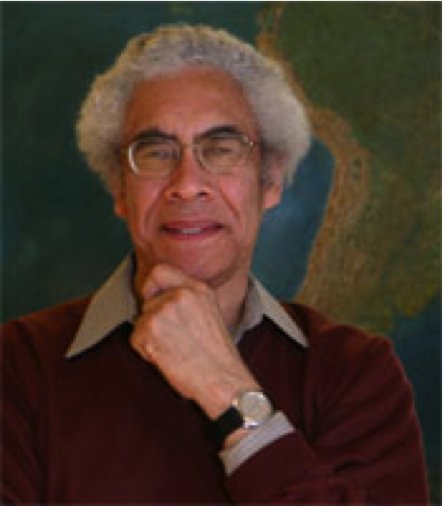
\includegraphics[width=4cm]{../figures/M1/philander}

\emph{\footnotesize{}\dots{} my story\textemdash{} disadvantaged in
South Africa, privileged in America\textemdash will interest readers
\dots{} }{\footnotesize\par}

\column{8cm}
\begin{itemize}
\item \emph{The \textquotedblleft time and chance\textquotedblright{} that
have happened to me personally over the past few decades may interest
a few young Africans, but they, unfortunately, are not avid readers
of Annual Reviews....}
\item continue on: \textbf{\textquotedblleft }\textbf{\uline{\href{https://www.researchgate.net/publication/228653879_Where_Are_You_From_Why_Are_You_Here_An_African_Perspective_on_Global_Warming}{Where Are You From? Why Are You Here? ...}}}\textbf{\textquotedblleft{}} 
\end{itemize}
\end{columns}

\end{frame}

%%%%
\begin{frame}{El Ni\~no and La Ni\~na}

\begin{columns}[t]

\column{8cm}

\emph{\tiny{In the year 1891, Se\~nor Dr. Luis Carranza, President
of the Lima Geographical Society, contributed a small article to the
Bulletin of that Society, calling attention to the fact that a counter-current
flowing from north to south had been observed between the ports of
Paita and Pacasmayo. The Paita sailors, who frequently navigate along
the coast in small craft, either to the north or the south of that
port, name this counter-current the current of El
Ni\~{n}o (the Child Jesus) because it has been observed
to appear immediately after Christmas. As this counter-current has
been noticed on different occasions, and its appearance along the
Peruvian coast has been concurrent with rains in latitudes where it
seldom if ever rains to any great extent, I wish, on the present occasion,
to call the attention of the distinguished geographers here assembled
to this phenomenon, which exercises, undoubtedly, a very great influence
over the climatic conditions of that part of the world.}}

\column{6cm}

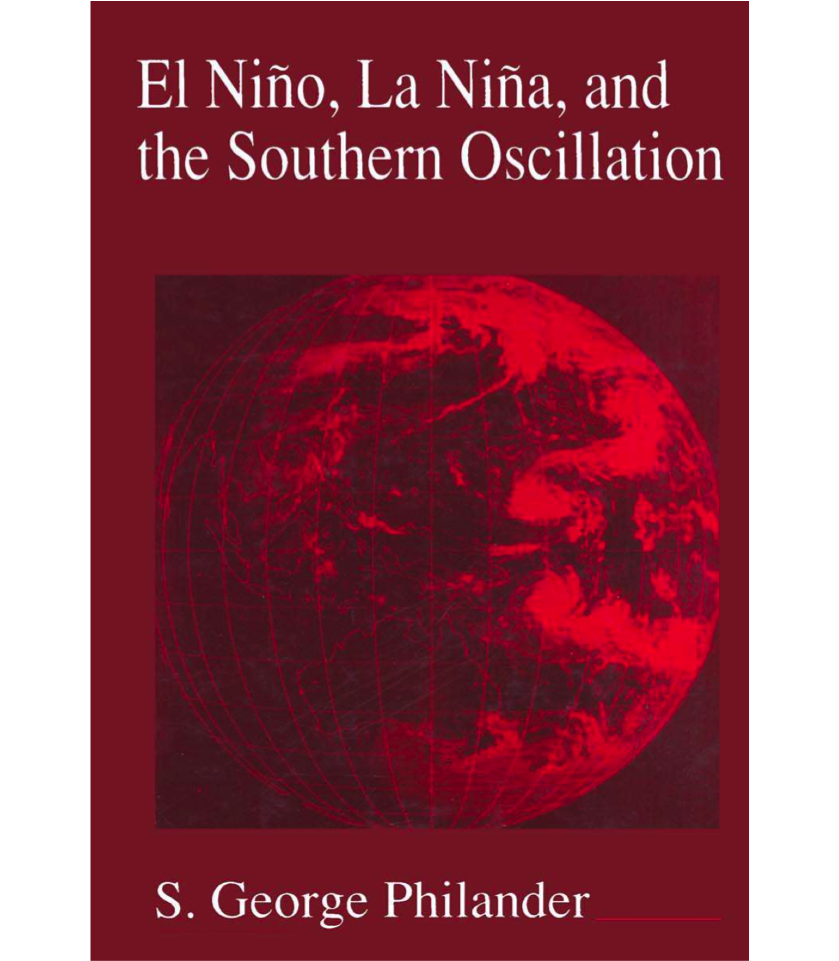
\includegraphics[width=5cm]{../figures/M1/philander_book}
\end{columns}

\end{frame}


%
\begin{frame}{The ``normal'' state...}
\begin{center}
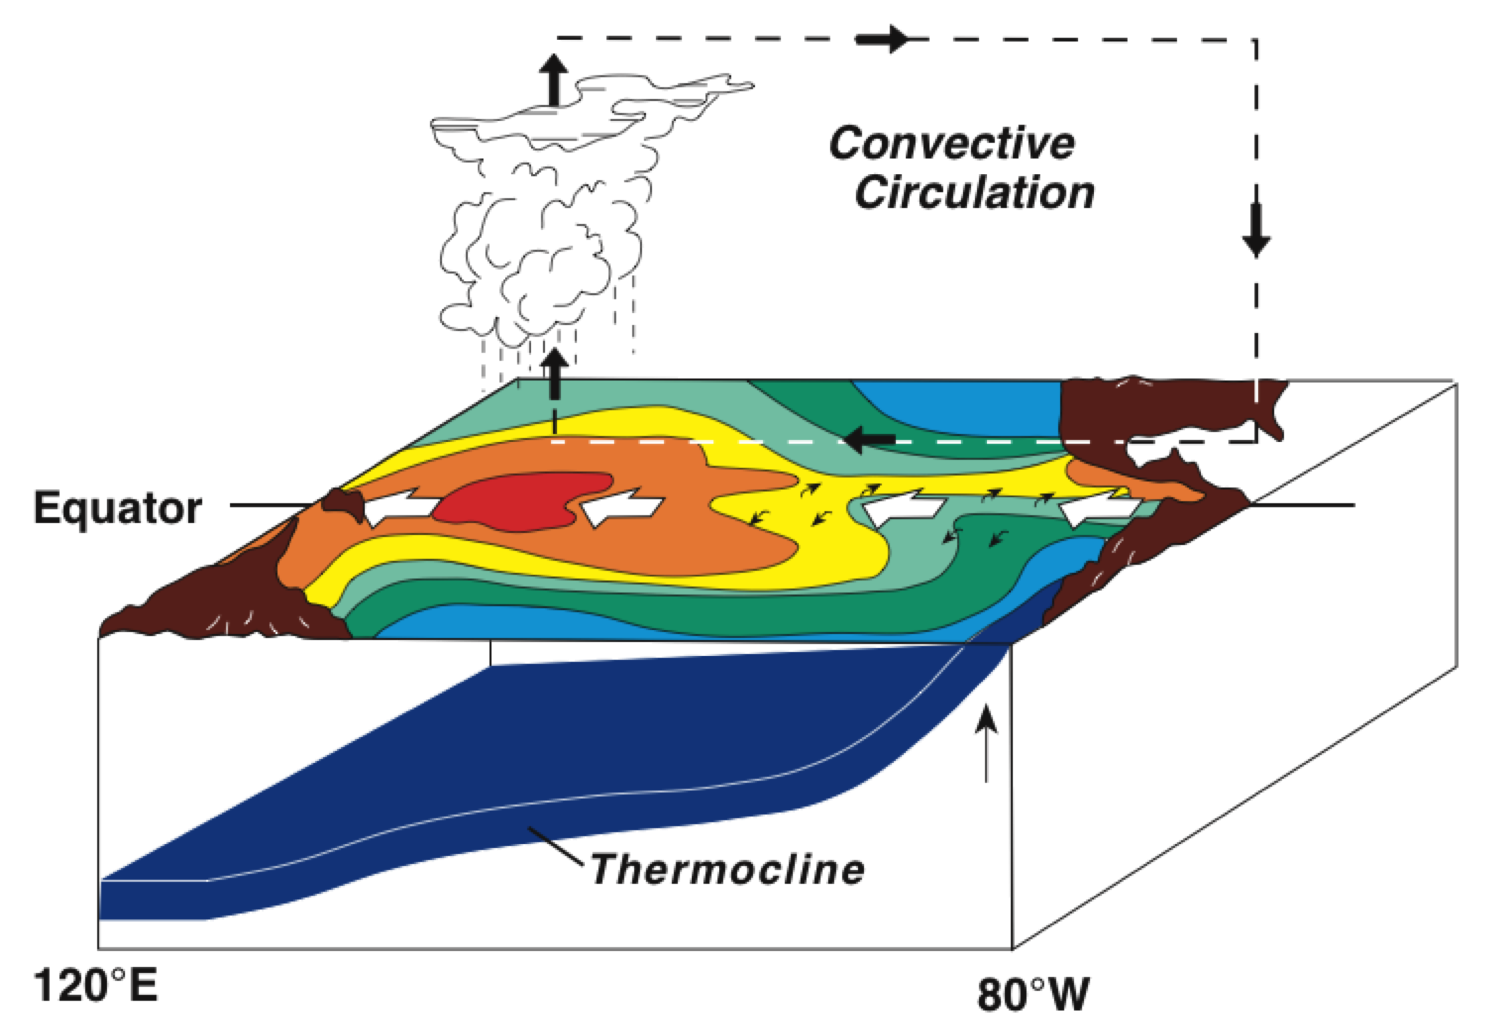
\includegraphics[scale=0.3]{../figures/M1/elnino_normal}
\par\end{center}

{\footnotesize{}... would persist if the equatorial ocean did not
respond to sudden changes in the wind, through the development of
large-scale propagating waves called }\textbf{\footnotesize{}Rossby}{\footnotesize{}
and }\textbf{\footnotesize{}Kelvin}{\footnotesize{} }\textbf{\footnotesize{}waves}{\footnotesize{}
(more of this in Module 6). These waves are }\textbf{\footnotesize{}solutions}{\footnotesize{}
of the shallow water equations, a special form of the equations of
}\textbf{\footnotesize{}geophysical fluid dynamics}{\footnotesize\par}

\end{frame}

\begin{frame}{Mathematics, scientific computing and ocean sciences}

\begin{itemize}
\item If you are a student of Science in the 21st century and you do not
use mathematical and computational tools, then you\textquoteright re
not doing science! (Glover et al., 2011)
\item Natural sciences have changed. We have moved from a \emph{descriptive}
era to a \emph{\emph{diagnostic and prognostic}} era, where the quantitative
knowledge of functions and processes in natural systems is necessary
to quantify the impacts of humans and on the future availability of
resources
\item From weather forecast, to environmental predictions and climate projections,
there is a need for \textbf{predictive models }based on quantitative
understanding of processes
\end{itemize}
\end{frame}

\begin{frame}{Mathematics and oceanography}


\framesubtitle{{\scriptsize{}This text has been rearranged from Cipra and Socha,
Mathematics and the ocean, 2001 (available in the course resources)} }
\begin{itemize}
\item Our understanding of the ocean has become increasingly scientific.
The observations of mariners throughout the ages have been augmented
by detailed measurements of water temperature and salinity, current
velocity, exchange of gas at the air-sea interface and spatial-temporal
distributions of marine life forms
\item Mathematics is the \textquotedblleft salty language\textquotedblright{}
of modern oceanography because it allows to quantify changes. Scientific
computing and computer visualization are the tools to \textquotedblleft speak
the language\textquotedblright{}
\item Observations often play a pivotal role but numerical models are nowadays
a fundamental workbench for understanding ocean and climate processes.
\emph{\small{}Future generations of oceanographer and climate scientists
must learn how to manage simple conceptual mathematical model first,
to appreciate the complex results of the modern numerical models (Drijfhout
et al., Ocean Circulation and Climate, Chapter 11, 2013).}{\small\par}
\end{itemize}
\end{frame}

\begin{frame}{Fluid dynamics}

\begin{columns}[t]


\column{8cm}
\begin{itemize}
\item {\footnotesize{}Fluid dynamics (or hydrodynamics) is a branch of applied
mathematics and engineering }{\footnotesize\par}
\item {\footnotesize{}It deals with the features of a fluid and its interactions
with structures or obstacles (fixed or time-varying). Fluid dynamics
is the basic science for areonautics, car manufacturing and all competitions
dealing with speed (F1, sailing, swimming, ...)}{\footnotesize\par}
\item {\footnotesize{}It is strongly grounded in computational mechanics
with complicated systems of differential equations. There is a major
assumption: }\textbf{\footnotesize{}the density of the fluid is constant}{\footnotesize{}
and depends on the fluid itself. It is a function of }\textbf{\footnotesize{}pressure}{\footnotesize{}
$\rho=\rho(p)$. }{\footnotesize\par}
\item {\footnotesize{}Pressure is a fundamental property in fluids. It expresses
the }\textbf{\footnotesize{}force exerted by a volume of fluid on
the surrounding, per unit of area}{\footnotesize{}. If pressure forces
are not balanced, we will have motion}{\footnotesize\par}
\end{itemize}

\column{6cm}

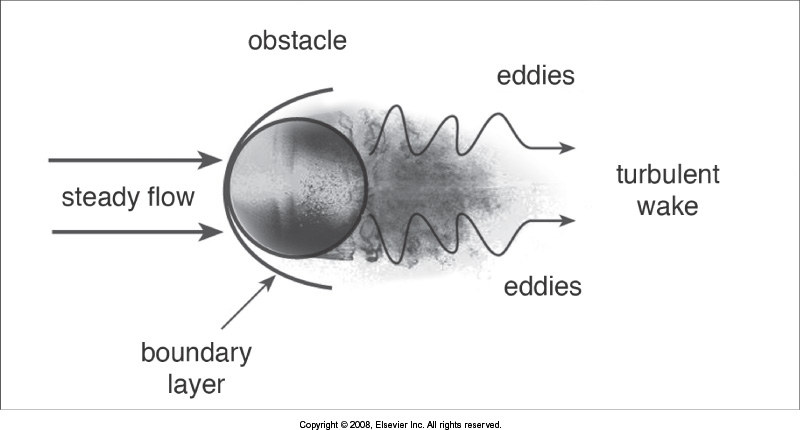
\includegraphics[width=6cm]{../figures/M1/MP-02}

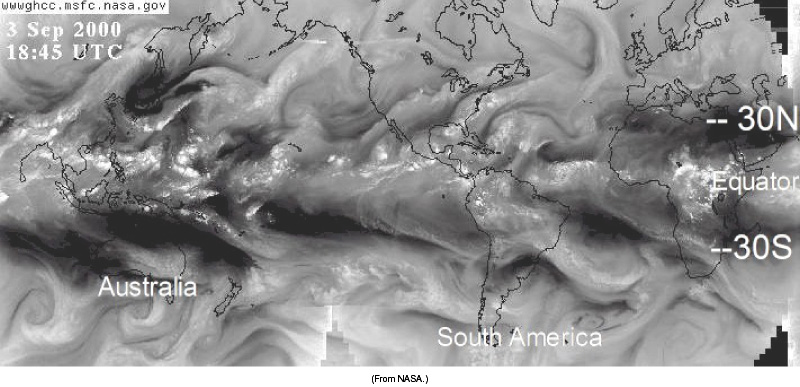
\includegraphics[width=6cm]{../figures/M1/MP-03}
\end{columns}

\end{frame}

\begin{frame}{Geophysical fluid dynamics}

\begin{columns}[t]


\column{7cm}
\begin{itemize}
\item {\footnotesize{}Natural fluids like the atmosphere and seawater are
also driven by pressure forces, but most of the energy has a thermal
origin and not mechanical.}{\footnotesize\par}
\item {\footnotesize{}An atmosphere where pressure is the only driver would
be a motionless and stable system. }{\footnotesize\par}
\item {\footnotesize{}In a fluid where $\rho=\rho(p,T,\ldots)$ there can
be heating of bottom layers from the Sun that generates movement called
}\textbf{\footnotesize{}convection}{\footnotesize{}: thermal energy
is converted to kinetic energy.}{\footnotesize\par}
\item {\footnotesize{}The motion of the fluid particles are then affected
by the}\textbf{\footnotesize{} Earth's rotation }{\footnotesize{}through
the Coriolis force}{\footnotesize\par}
\item {\footnotesize{}Ocean and atmosphere are described by }\textbf{\footnotesize{}geophysical
fluid dynamics (GFD)}{\footnotesize\par}
\end{itemize}

\column{6cm}

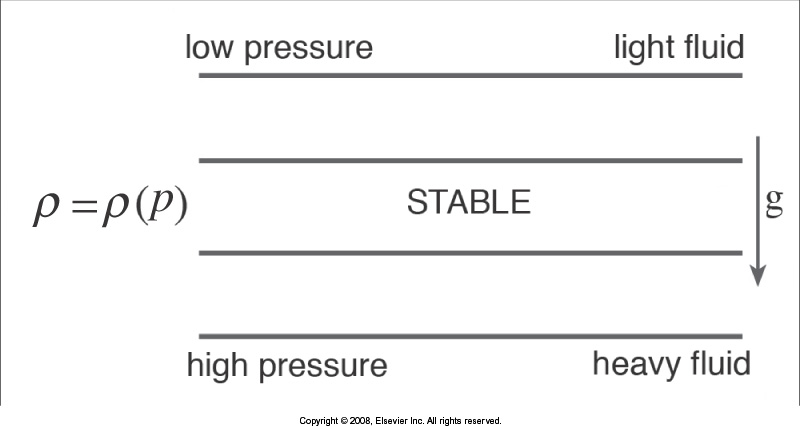
\includegraphics[width=6cm]{../figures/M1/MP-04}

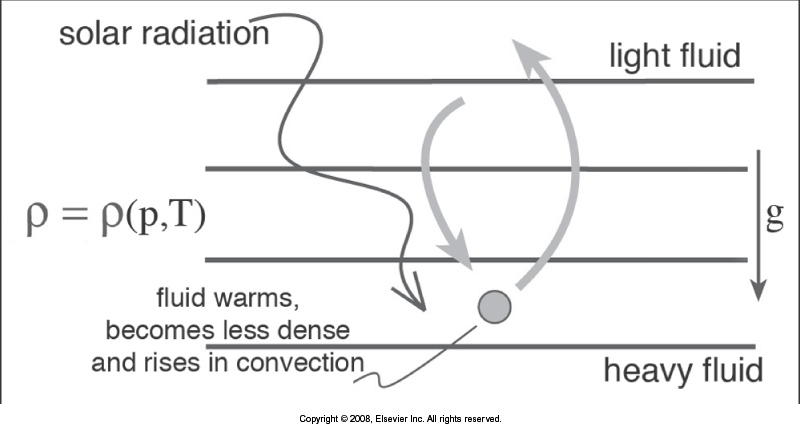
\includegraphics[width=6cm]{../figures/M1/MP-05}
\end{columns}

\end{frame}

\begin{frame}{An example of GFD at work: wild fire in the Cape Peninsula (March
2015)}

\centering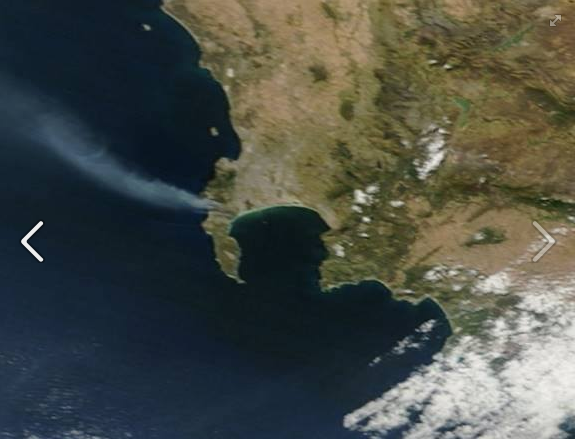
\includegraphics[scale=0.5]{../figures/M1/capetown_fire_sat}
\end{frame}

\begin{frame}{What governs the motion: advection-diffusion-reaction equation}

\begin{example}
The dynamics of a tracer in the ocean or in the air, like the concentration
of pollutants at a river mouth or smoke from a fire are described
through dynamical Partial Differential equations (PDE) 
\[
\frac{\partial\psi\left(\mathbf{x},t\right)}{\partial t}=A\left(\mathbf{x},t\right)+D\left(\mathbf{x},t\right)+R\left(\mathbf{x},t\right)
\]
\end{example}

\begin{columns}[t]


\column{8cm}
\begin{itemize}
\item We will derive this equation from first principles of energy and mass
conservation. The one-dimensional form is written as
\[
\frac{\partial\psi}{\partial t}=-u\frac{\partial\psi}{\partial x}+\frac{\partial}{\partial x}\left(D\frac{\partial\psi}{\partial x}\right)+R\left\{ \frac{d\psi}{dt}\right\} 
\]
\end{itemize}

\column{4cm}

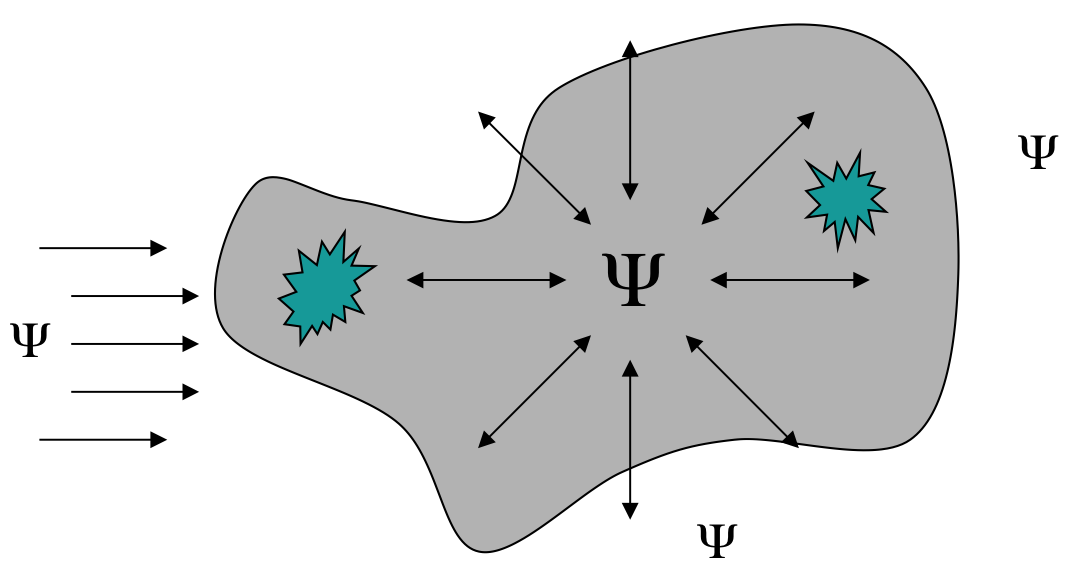
\includegraphics[scale=0.25]{../figures/M1/PDE_tracer_ADR}
\end{columns}

\end{frame}

\begin{frame}{The basic equations of geophysical fluid dynamics}

\begin{columns}[c]


\column{6cm}
\begin{itemize}
\item The \textbf{Navier-Stokes equations} are the \textbf{primitive} equations
of GFD
\item They describe the conservation of mass and momentum for an infinitesimal
water parcel in the water, which is treated as a \emph{continuum}.
They derive strictly from Newton's laws.
\item Cannot be solved analytically (one of the Millenium problems, worth
\$1M)
\end{itemize}

\column{6cm}

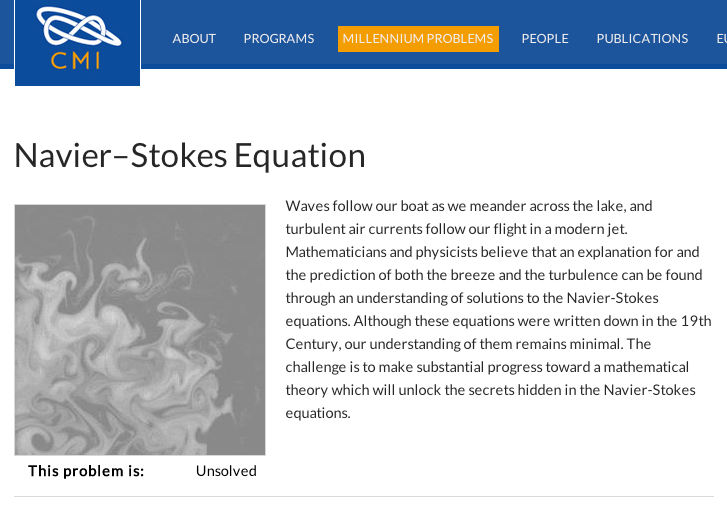
\includegraphics[scale=0.25]{../figures/M1/N-S_millenium}
\end{columns}

\end{frame}

\begin{frame}{Laboratory experiments in geophysical fluid dynamics}

\begin{columns}[c]


\column{7cm}
\begin{itemize}
\item Most of the geophysical fluid dynamics processes are scalable, which
means that certain equilibria that are observed at planetary scales
can be reproduced in an appropriate laboratory setup
\item These experiments can be done using a rotating tank, to simulate the
rotation of the Earth
\item The biggest turntable in the world is at \uline{\href{http://www.legi.grenoble-inp.fr/web/spip.php?article757&lang=en}{LEGI}},
in Grenoble (in French, check the 3D virtual tour)
\end{itemize}

\column{6cm}

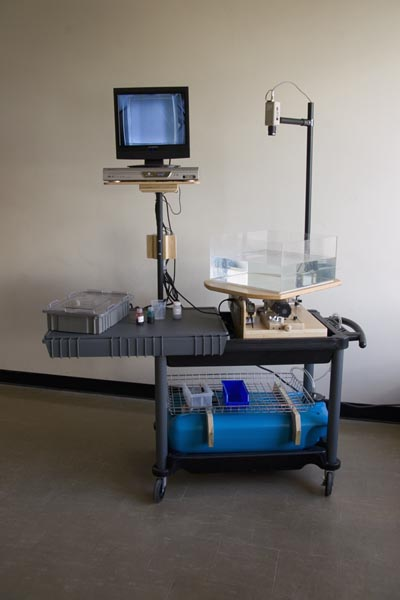
\includegraphics[scale=0.5]{../figures/M1/Turntable_Cart}
\end{columns}

\end{frame}


\section{Linear algebra: a primer}
\begin{frame}{Scalars, vectors and matrices}

\begin{definitions}
{\small{}A }\textbf{\small{}scalar}{\small{} is a single number (or
a bunch of), usually indicated with a latin or greek symbol $a$,
$\phi$. A }\textbf{\small{}vector}{\small{} is an }\textbf{\small{}ordered}{\small{}
row or column of numbers, usually indicated with a letter and an arrow
$\vec{a}$, a bold lowercase letter $\boldsymbol{a}$, or a letter
with one index $a_{i}$. A }\textbf{\small{}matrix}{\small{} is a
bundle of scalars or vectors; it can be a flat combination of rows
and columns (a 2-D matrix, indicated with a bold capital letter }\textbf{\small{}$\boldsymbol{A}$}{\small{}
or with a letter and 2 indices $a_{ij}$) or a multidimensional }\textbf{\small{}array}{\small{}
(a vector is a 1-D array; 3-D arrays are indicated with multiple indices
$a_{ijk}$, and so on)}{\small\par}
\end{definitions}

\begin{itemize}
\item {\small{}This is the simple algebraic definition, but what really
matters is what every entity represents in a physical sense}

\begin{itemize}
\item {\small{}a scalar is a quantity identifiable only with }\textbf{\small{}magnitude}{\small{}
(e.g. temperature, pressure, nutrient concentration, etc.)}{\small\par}
\item {\small{}a vector carries information on }\textbf{\small{}both direction
and magnitude}{\small{} (e.g. winds or currents)}{\small\par}
\item {\small{}a matrix (also called a tensor) provides information in a
}\textbf{\small{}multi-dimensional space}{\small{} (the term space
should be considered in an abstract way)}{\small\par}
\end{itemize}
\end{itemize}
\end{frame}

\begin{frame}{Scalar fields in ocean and atmosphere sciences}

\begin{itemize}
\item The typical scalar variables are temperature, wind, pressure, humidity, irradiance, precipitation, salinity, nutrient concentrations, abundance of organisms, etc. 
\item \textbf{Scalar fields} are \textbf{multidimensional objects}: containers of values at certain points in space and time: $T(x,y,z,t)$
\item 2-D scalar fields are represented with contour lines or shadings (heat maps)
\end{itemize}
\end{frame}


%%%%%%%%%%%%%%%%%%%%%%%
\begin{frame}{Examples of scalar variables (time series)}

\begin{columns}[c]

\column{9cm}
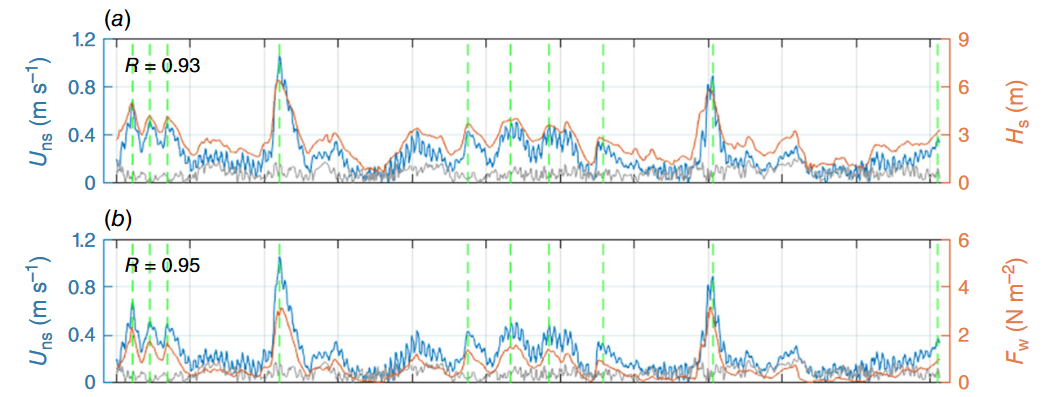
\includegraphics[width=9cm]{figures/M1/timeseries.png}

\column{6cm}
\begin{itemize}
\item a \textbf{time series} is the time evolution of a scalar field at
a fixed position, $T(x_{0},y_{0},z_{0},t)=f\left(t\right)$
\item Simulated time series of near surface current speeds (left-hand y-axes) plotted against (a) significant wave height (Hs), (b) wave-induced force (Fw) (de Vos et al., 2023).
\item Produced with Matlab. \textbf{Q: what is missing in this plot?}
\end{itemize}

\end{columns}

\end{frame}

%%%%%%%%%%%%%%%%%%%%%%%
\begin{frame}{Examples of scalar  (profiles)}

\begin{columns}[c]

\column{9cm}
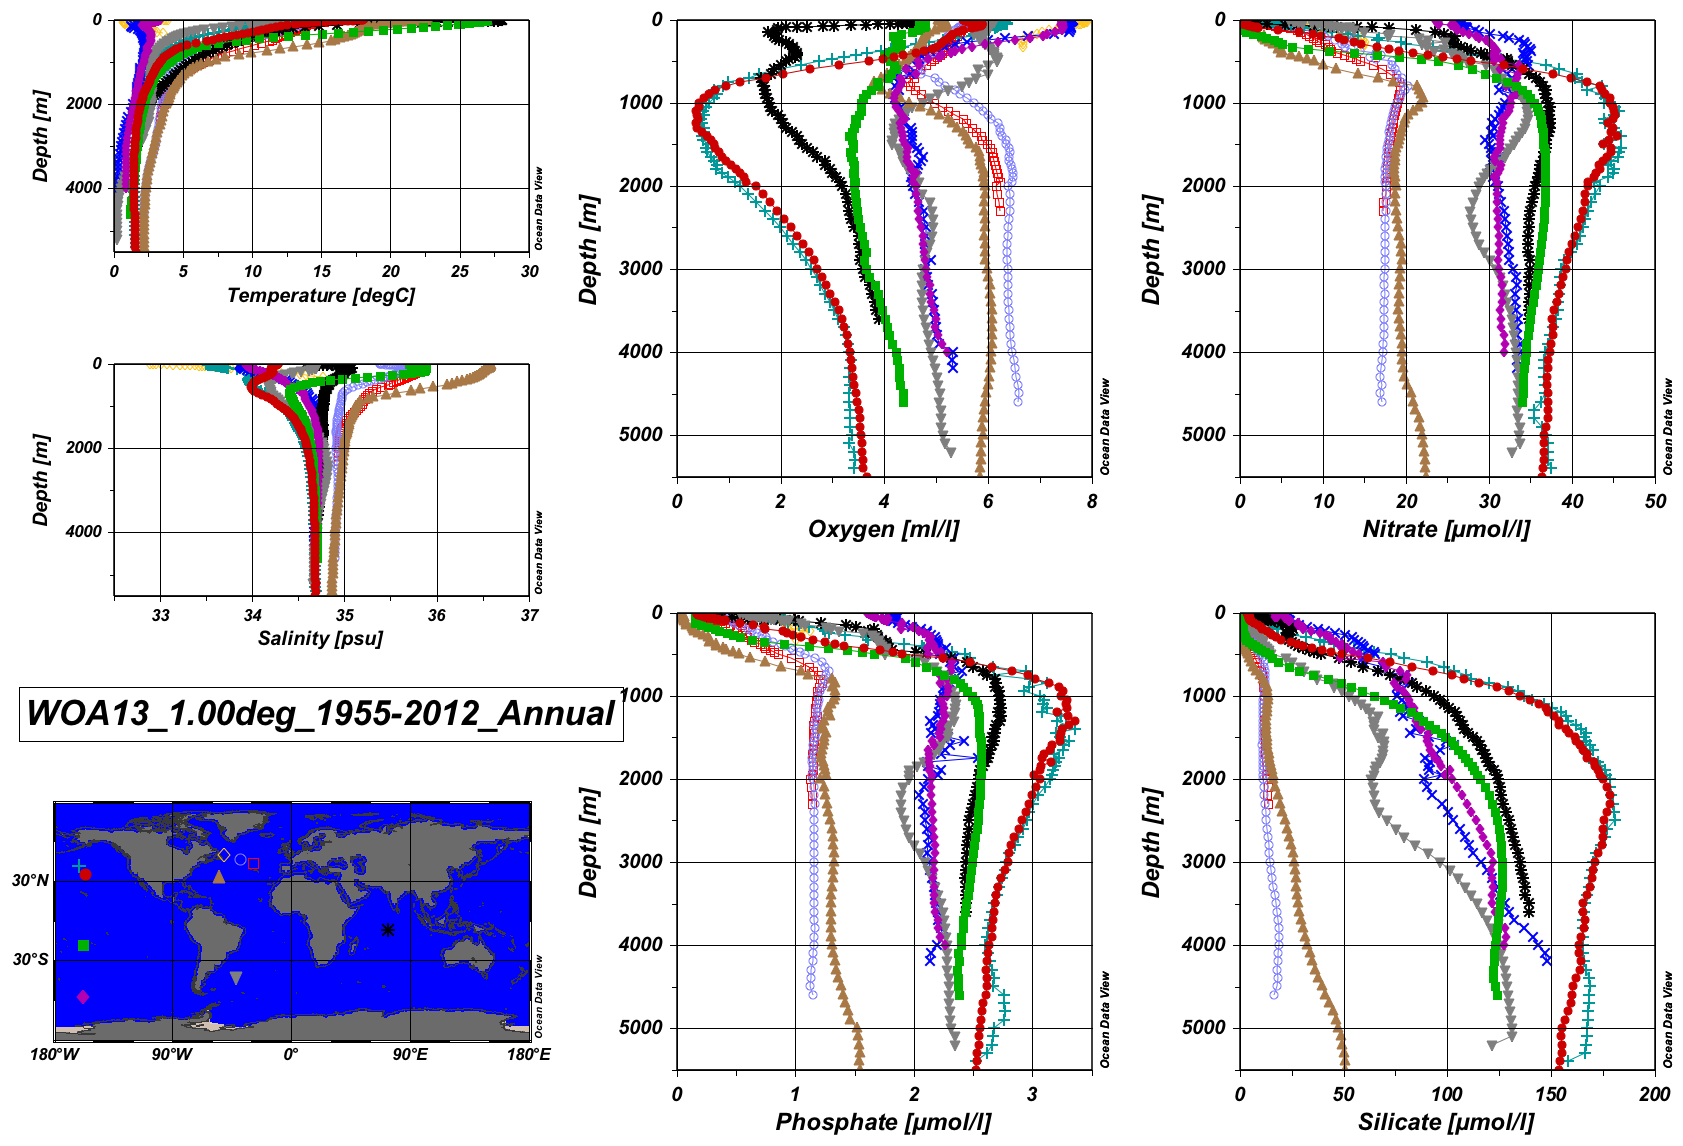
\includegraphics[width=9cm]{../figures/M1/Profiles_WOA13_ODV}

\column{6cm}
\begin{itemize}
\item a \textbf{profile} shows the field in the vertical dimension at a fixed moment in time $T(x_{0},y_{0},z,t_{0})=f\left(z\right)$ 
\item Depth profiles at various points in the world ocean from the World
Ocean Atlas gridded dataset
\item Produced with Ocean Data View
\end{itemize}

\end{columns}

\end{frame}


\begin{frame}{Examples of scalar 2-D fields (maps)}

\begin{columns}[c]

\column{9cm}

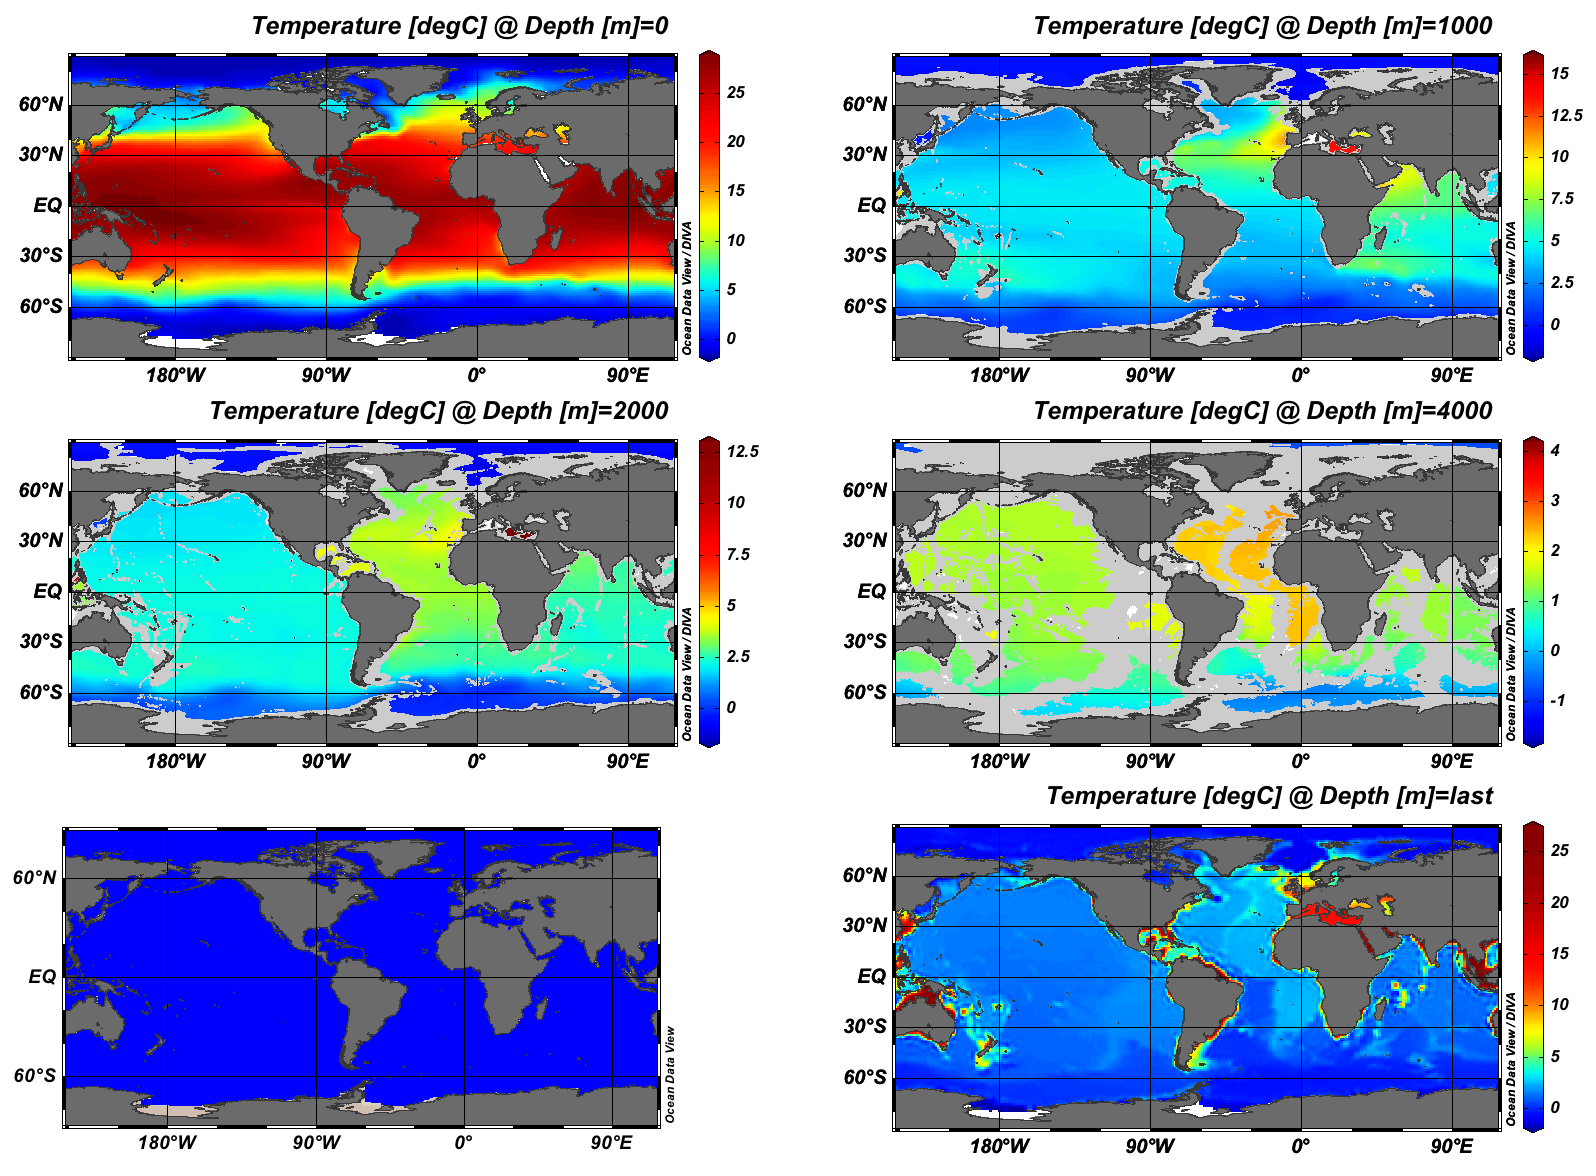
\includegraphics[width=9cm]{../figures/M1/Temperature_maps_WOA13_ODV}

\column{5cm}
\begin{itemize}
\item Horizontal slices at a given time $T(x,y,z_{0},t_{0})=f\left(x,y\right)$
are called \textbf{maps}
\item Temperature maps at various depth from the World Ocean Atlas
gridded dataset. The first 4 graphs are slices at given depths; the last one is
an \emph{isosurface} at the bottom 
\item Produced with Ocean Data View
\end{itemize}
\end{columns}

\end{frame}

\begin{frame}{Examples of scalar 2-D biogeochemical fields (maps)}

\begin{columns}[c]


\column{7cm}

\vspace{-0.5cm}
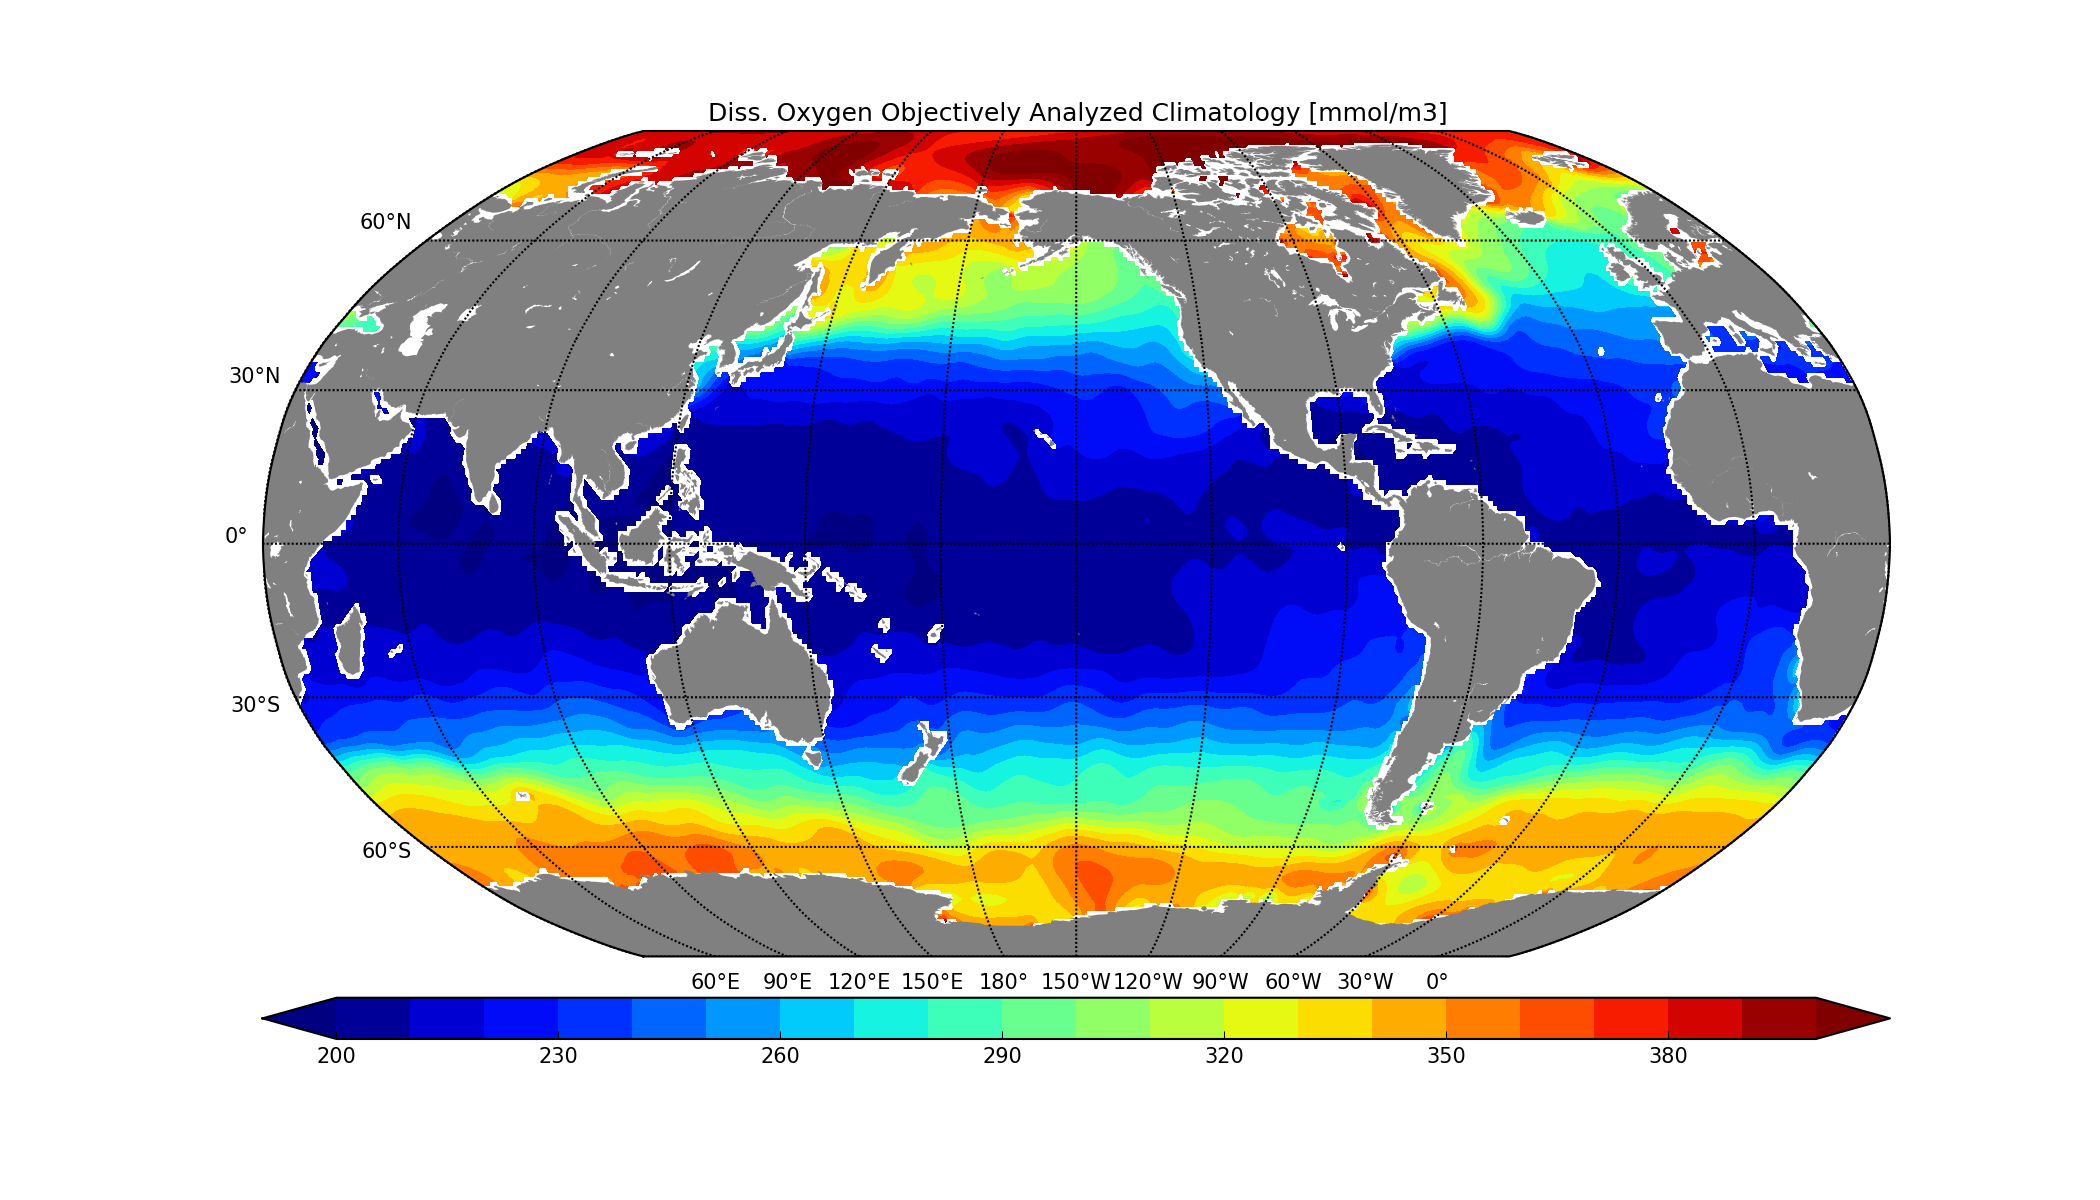
\includegraphics[width=6cm]{../figures/M1/Oxygen_map_WOA9_python}

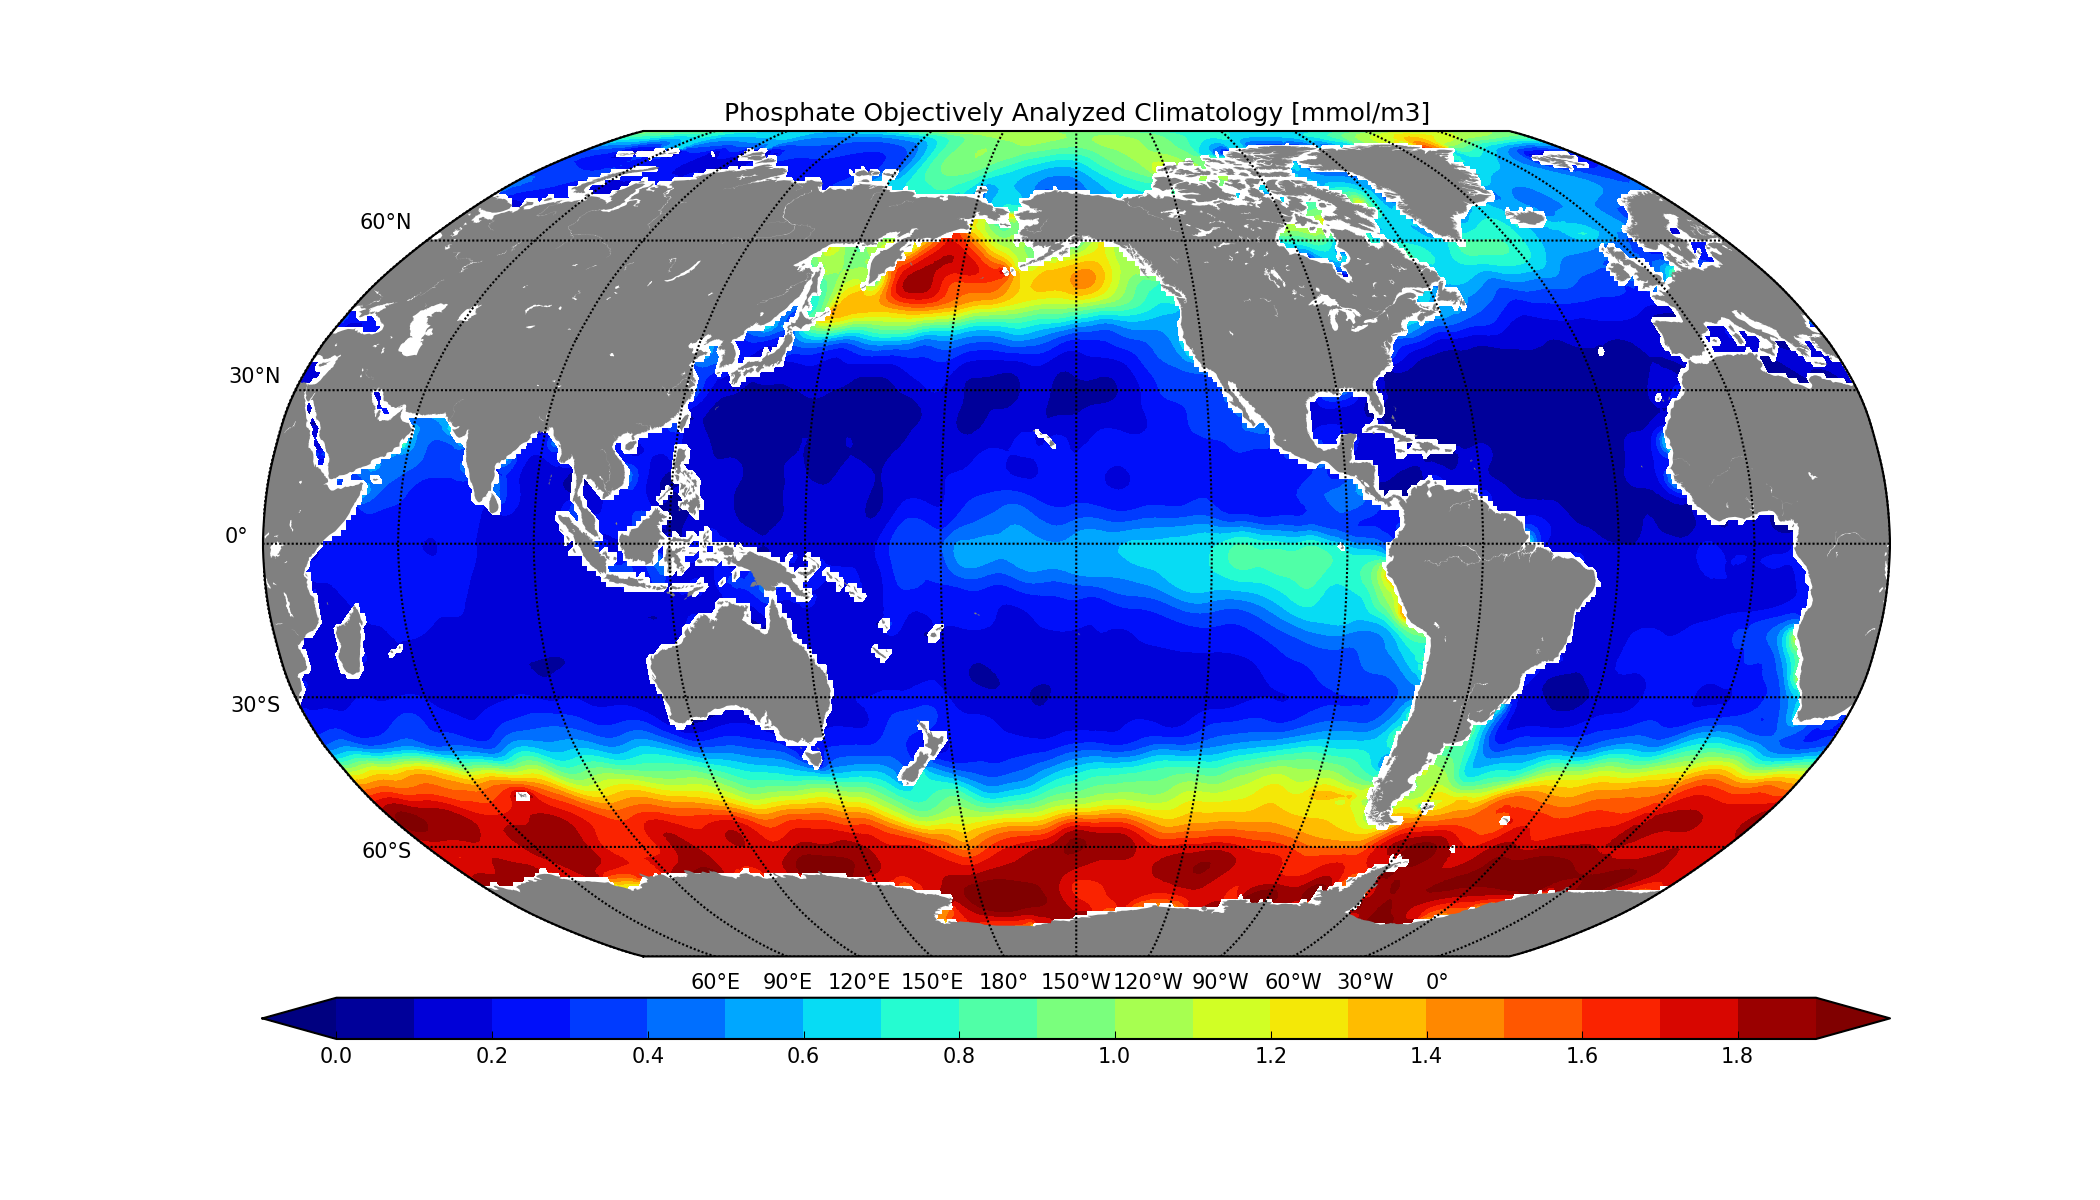
\includegraphics[width=6cm]{../figures/M1/Phosphate_map_WOA9_python}

\column{6cm}
\begin{itemize}
\item Surface mean annual concentrations of oxygen and phosphate from the
World Ocean Atlas gridded dataset
\item This is a contour filled plot. The colormap is discretized and it is
easier to read the values
\item Produced with python 
\end{itemize}
\end{columns}

\end{frame}

\begin{frame}{Examples of scalar fields (sections)}

\begin{columns}[c]

\column{9cm}
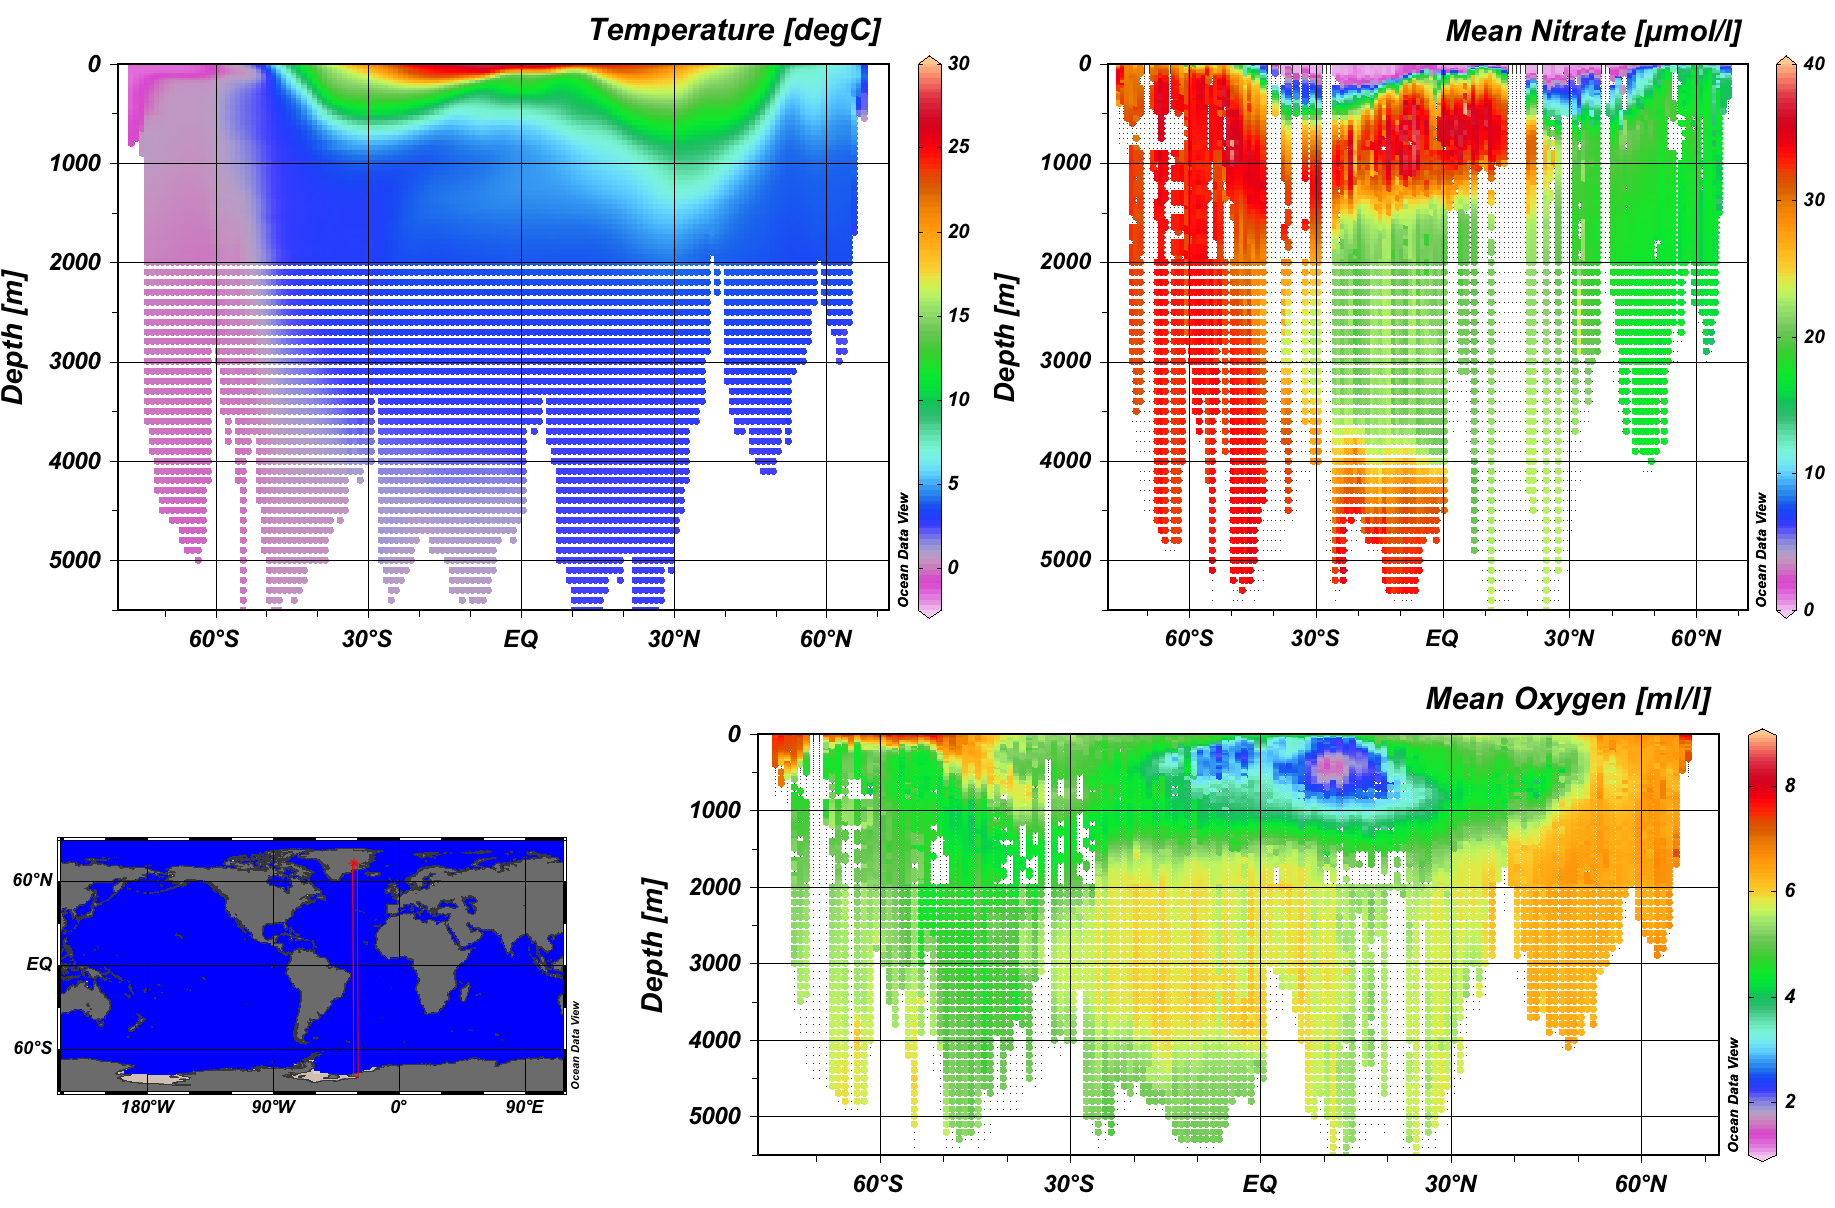
\includegraphics[width=9cm]{../figures/M1/Sections_WOA13_ODV}

\column{5cm}
\begin{itemize}
\item Vertical slices $T(x,y_{0},z,t_{0})$
or $T(x_{0},y,z,t_{0})$ are called \textbf{sections }(zonal and meridional,
respectively)
\item Temperature, Nitrate and oxygen concentration in the Atlantic from
the World Ocean Atlas gridded dataset
\item Produced with Ocean Data View
\end{itemize}
\end{columns}

\end{frame}

\begin{frame}{The H\"ovm\"oller plot: mixing time and space}

\begin{center}
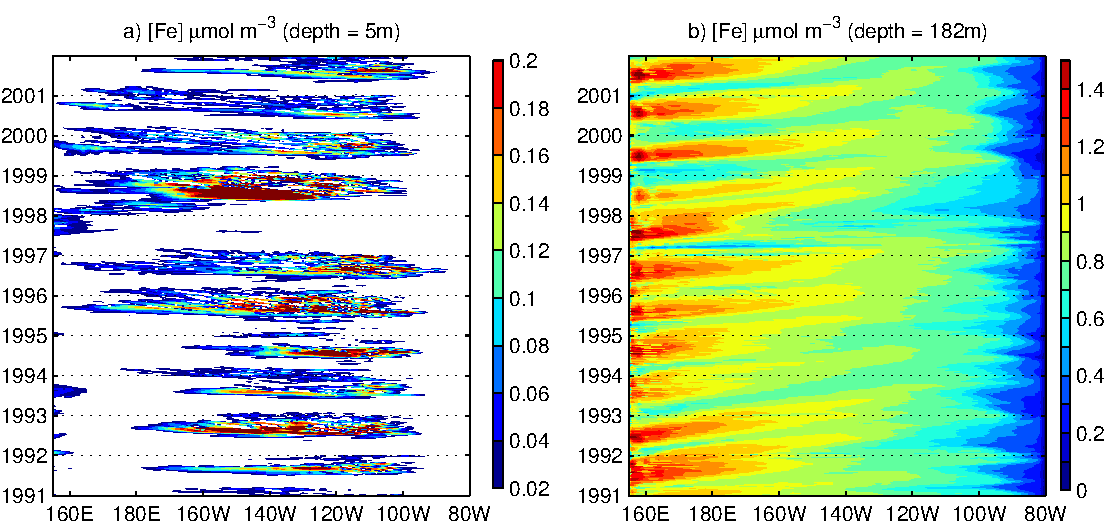
\includegraphics[width=9cm]{../figures/M1/Hoevmoeller_PELAGOS_matlab}
\par\end{center}
\begin{itemize}
\item \small{The combination of time and space coordinates gives a special map
called H\"ovm\"oller plot (typically $T(x,y_{0},z_{0},t)$
or $T(x_{0},y,z_{0},t)$)}
\item \footnotesize{Iron concentration at surface and in the Equatorial Undercurrent (EUC) in the Pacific Ocean at the equator. The slope of the stripes indicate the speed of the EUC th   at carries Fe to the Eastern Pacific.}
\item \footnotesize{Produced with Matlab} 
\end{itemize}
\end{frame}


\section{Vectors}
\begin{frame}{Vectors in ocean and atmosphere science}

\begin{itemize}
\item The typical vector fields are wind or current velocities. They are
expressed in terms of components along the 3 spatial dimensions: $\vec{U}=\mathbf{U}=\left(u,v,w\right)$ 
\item Operations on vectors and scalars (see next lecture notes) may lead
to the following \textbf{space operators}:

\begin{itemize}
\item Some derived quantities from scalar fields are also vectors: \textbf{the
gradient} (the pressure gradient)
\item Some derived quantities from vector fields are scalars: \textbf{the
divergence }(the fluid divergence)
\item Some derived quantities from vector fields are vectors: \textbf{the
curl }(the wind stress curl)
\end{itemize}
\end{itemize}
\end{frame}

\begin{frame}{Atmospheric fields: wind stress}
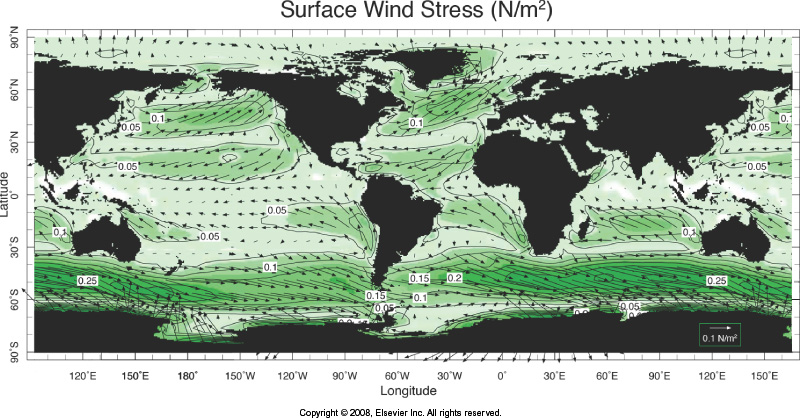
\includegraphics[scale=0.4]{../figures/M1/MP_10_02_wstress}

Wind stress intensity (scalar) and wind vectors (Marshall and Plumb,
Fig. 10.2)
\end{frame}

\begin{frame}{Examples of oceanic vector fields}
\begin{columns}[t]

\column{8cm}
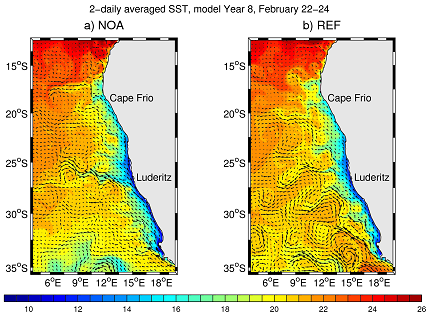
\includegraphics[width=8cm]{../figures/M1/vector_noagulhas}

\column{4cm}
\begin{itemize}
\item Simulated SST (scalar field) with surface current vectors overlaid
for (a) a model experiment in which the effect of the Agulhas has
been removed and (b) for the 'realistic' case
\item From J. Veitch's PhD thesis (done with Matlab)
\end{itemize}
\end{columns}

\end{frame}


\begin{frame}{Vectors in maths}
\framesubtitle{Practical: Chapter 4, C. Moler, Experiments with Matlab, http://www.mathworks.com/moler/exm,
free e-book}
\begin{definition}
\textbf{Linear algebra} is the branch of mathematics that deals with
vectors and matrices 
\end{definition}

\begin{columns}[t]

\column{8cm}
\begin{itemize}
\item {\footnotesize{}The most simple example of a vector is expressed by
the coordinates of a point on the Cartesian plane. The point is indicated
by a column vector with 2 components (or elements), one for each coordinate.
They are grouped with brackets. It is customary to indicate a point
with $\left(\right) \, \left[\right]$, and the components of a vector with $\left\langle \right\rangle $ }{\footnotesize\par}
\item {\footnotesize{}Note that there is no limit to the number of components.
Vectors in physics are intuitively linked to spatial (+ time) dimensions
but they have to be thought as abstract data structures very useful
for scientific computing (called}\textbf{\footnotesize{} ARRAYS}{\footnotesize{})}{\footnotesize\par}
\end{itemize}

\column{6cm}

{\footnotesize{}
\[
x_{i}=\mathbf{x}=\begin{pmatrix}x_{1}\\
x_{2}
\end{pmatrix}=\begin{bmatrix}x_{1}\\
x_{2}
\end{bmatrix}=\left\langle \begin{array}{c}
x_{1}\\
x_{2}
\end{array}\right\rangle 
\]
}{\footnotesize\par}

{\footnotesize{}
\[
v_{i}=\begin{pmatrix}v_{1}\\
v_{2}\\
v_{3}\\
\vdots\\
v_{n}
\end{pmatrix}
\]
}{\footnotesize\par}
\end{columns}

\end{frame}

\begin{frame}{Vectors in the 3-dimensional space}

\begin{columns}[t]


\column{8cm}
\begin{itemize}
\item {\small{}A point in the 3-dimensional Cartesian space is a}\textbf{\small{}
positional vector}{\small{}: in the example on the right, the vector
$\boldsymbol{a}$ connects the origin of the system to the point (the
tip of the arrow). It will have 3 components, the values of the coordinates
along the $x$, $y$ and $z$ axes}{\small\par}
\item \textbf{\small{}The Cartesian axes are vectors themselves}{\small{}:
unit vectors or direction vectors}{\small\par}
\item {\small{}A vector in space is uniquely determined by an origin (the
tail), and a triplet of components (that locate the tip). They must
be referenced to a system of coordinates which is itself a triplet
of unit vectors }{\small\par}
\item {\small{}\url{https://www.intmath.com/vectors/3d-space-interactive-applet.php}}{\small\par}
\end{itemize}

\column{5.5cm}

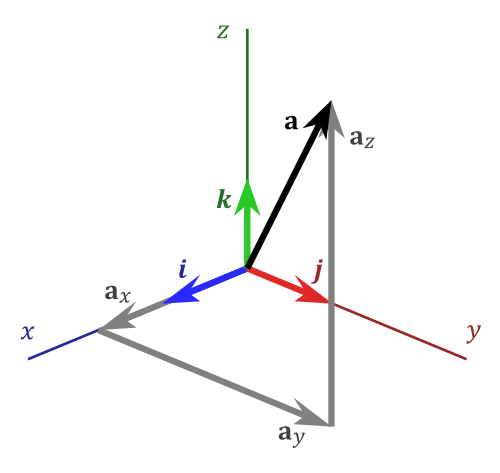
\includegraphics[scale=0.3]{../figures/M1/3D_Vector_versor}\\
Every point is a vector: 

$\vec{a}=\mathbf{a}=\left(a_{1},a_{2},a_{3}\right)=\left(a_{x},a_{y},a_{z}\right)\Rightarrow a_{x}\mathbf{\hat{i}}+a_{y}\mathbf{\hat{j}}+a_{z}\mathbf{\hat{k}}$ 
\end{columns}

\end{frame}

\begin{frame}{Vector components}
\begin{columns}[t]

\column{7cm}

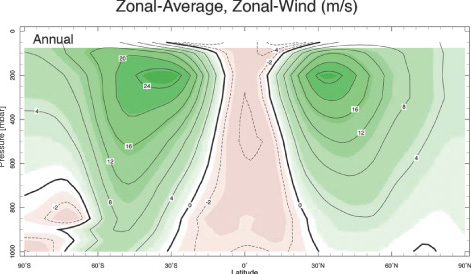
\includegraphics[clip,scale=0.45]{../figures/M1/MP-5_20_zonal_winds}

\column{6cm}
\begin{itemize}
\item Vectors have \textbf{sense} (the arrow), \textbf{direction} (the line), and \textbf{magnitude} (the line's length). \uline{The components of a vector are scalars}, and you can plot them for each direction.
\item \small{Annual \textbf{zonal} mean of the \textbf{wind zonal component} as
a function of height. The two mid-latitude jet streams are visible,
as well as the major structures of Easterlies and Westerlies in the
lower troposphere (from Marshall and Plumb Fig. 5.20)}
\end{itemize}
\end{columns}

\end{frame}

\begin{frame}{Vector \emph{sense}, addition, and subtraction}

\begin{itemize}
\item The negative of a vector has the opposite sense: same magnitude but negative components
\item The sum of 2 vectors is the sum of the elements and \textbf{the result
is a vector}
\[
\mathbf{x}+\mathbf{y}=\begin{bmatrix}x_{1} & x_{2} & x_{3}\end{bmatrix}+\begin{bmatrix}y_{1} & y_{2} & y_{3}\end{bmatrix}=\begin{bmatrix}x_{1}+y_{1} & x_{2}+y_{2} & x_{3}+y_{3}\end{bmatrix}
\]
It is geometrically interpreted as the \emph{parallelogram} combination
of the two vectors when connected by the tails
\end{itemize}
\begin{columns}[c]
  \begin{column}{0.5\textwidth}
    \centering
    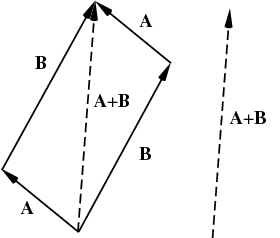
\includegraphics[scale=0.4]{../figures/M1/ParallelogramLaw}
  \end{column}
  \begin{column}{0.5\textwidth}
    \footnotesize{ \textbf{Questions}: 
    \begin{enumerate}
        \item What happens if the two vectors are at a right angle?
        \item How do you compute the difference?
        \item What is the result if you multiply a vector by a scalar?
    \end{enumerate}}
  \end{column}
\end{columns}
\end{frame}


\section{Matrices}
\begin{frame}{Matrices in math}

\begin{tikzpicture}[remember picture,overlay]
\node at (2,-3) {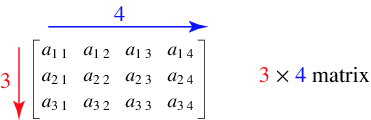
\includegraphics[scale=0.3]{../figures/M1/Matrix_3x4}};
\end{tikzpicture}
\begin{itemize}
\item A matrix is an \textbf{ordered arrangement} of row and column vectors
\item An $m\times n$ matrix consists of $m$ rows and $n$ columns (counting
from the upper left corner)
\item Any element of the matrix is identified with a pair of indices corresponding
to the row and column numbers
\[
\mathbf{A}=A_{ij}=\begin{bmatrix}a_{11} & a_{12} & a_{13}\\
a_{21} & a_{22} & a_{23}\\
a_{31} & a_{32} & a_{33}
\end{bmatrix}
\]
\item A matrix is called \textbf{square} when the number of rows equals
the number of columns
\item {\small{}There can be 0s in a matrix (if all, it's the zero matrix).
A matrix with all 0s except on the diagonal is a }\textbf{\small{}diagonal
matrix}{\small{} (it's a square matrix!). 
\[
\begin{bmatrix}a_{11} & 0 & 0\\
0 & a_{22} & 0\\
0 & 0 & a_{33}
\end{bmatrix}
\]
}{\small\par}
\end{itemize}
\end{frame}

\begin{frame}{The identity matrix}
\begin{itemize}
\item {\footnotesize{}The }\textbf{\footnotesize{}identity matrix}{\footnotesize{}
$I$ is the equivalent of ``1'' in algebra. It is a diagonal matrix
with 1s on the diagonal and it can be of any dimension
\begin{equation}
\mathbf{I}=\begin{bmatrix}1 & 0 & 0\\
0 & 1 & 0\\
0 & 0 & 1
\end{bmatrix}\label{eq:identity-matrix}
\end{equation}
}{\footnotesize\par}
\item {\footnotesize{}In the 3-D space, the identity matrix }\textbf{\footnotesize{}identifies
the Cartesian system of coordinates}{\footnotesize{}, because each
row or column represents the unit vector for each direction (called
}\emph{\footnotesize{}bases}{\footnotesize{})
\[
\mathbf{\hat{i}}=\begin{bmatrix}1\\
0\\
0
\end{bmatrix};\ \mathbf{\hat{j}}=\begin{bmatrix}0\\
1\\
0
\end{bmatrix};\ \mathbf{\hat{k}}=\begin{bmatrix}0\\
0\\
1
\end{bmatrix}
\]
}{\footnotesize\par}
\end{itemize}
\begin{columns}[c]

\column{10cm}
\begin{itemize}
\item {\footnotesize{}This matrix has a lot of interesting properties: it
is }\emph{\footnotesize{}orthogonal}{\footnotesize{} because all the
vectors are at right angles to each other, and all vectors are of
length (}\emph{\footnotesize{}magnitude or norm}{\footnotesize{})
1: $\left\Vert \mathbf{\hat{i}}\right\Vert =\sqrt{1^{2}+0^{2}+0^{2}}=1$.
All systems of coordinates must be }\emph{\footnotesize{}ortho-normal}{\footnotesize{}.
It is also the only matrix that does not change when it is }\emph{\footnotesize{}transposed}{\footnotesize{},
that is rows and columns are swapped $\mathbf{I}^{T}=\mathbf{I}$
(}\textbf{\footnotesize{}note:}{\footnotesize{} the transpose of a
matrix is not the inverse!)}{\footnotesize\par}
\end{itemize}

\column{4cm}

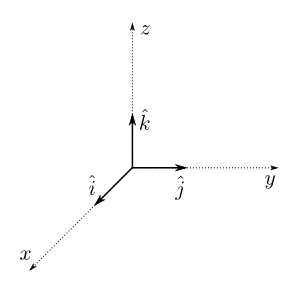
\includegraphics[width=3cm]{../figures/M1/Unit-vectors-in-Cartesian-Coord}
\end{columns}

\end{frame}

\begin{frame}{Operations with vectors and matrices}

\begin{itemize}
\item Arithmetic operators (sum and difference)q are applied quite naturally
to vectors/matrices, \textbf{provided that they are of the same size!}
The same for the multiplication by a scalar\footnote{In math, there is usually no  operator for the multiplication}
\item They are all performed element-by-element
\begin{align*}
\mathbf{x}+\mathbf{y} & =\begin{pmatrix}x_{1}\\
x_{2}
\end{pmatrix}+\begin{pmatrix}y_{1}\\
y_{2}
\end{pmatrix}=\begin{pmatrix}x_{1}+y_{1}\\
x_{2}+y_{2}
\end{pmatrix}\\
\mathbf{A}-\mathbf{B} & =\begin{bmatrix}a_{11} & a_{12}\\
a_{21} & a_{22}
\end{bmatrix}-\begin{bmatrix}b_{11} & b_{12}\\
b_{21} & b_{22}
\end{bmatrix}=\begin{bmatrix}a_{11}-b_{11} & a_{12}-b_{12}\\
a_{21}-b_{21} & a_{22}-b_{22}
\end{bmatrix}\\
s\mathbf{x} & =\begin{pmatrix}sx_{1}\\
sx_{2}
\end{pmatrix}\\
k\mathbf{A} & =\begin{bmatrix}ka_{11} & ka_{12}\\
ka_{21} & ka_{22}
\end{bmatrix}
\end{align*}
\end{itemize}
\end{frame}

\begin{frame}{Matrix multiplication (I)}

\begin{itemize}
\item \emph{If you are unfamiliar with matrices, do the Kahn Academy section
first!} One way to understand matrix multiplication is to think of
systems of coordinates 
\item Any number can be seen as the product of itself by 1, as well as any
vector in the 3-D system can be seen as the matrix product of itself
by the identity matrix. This operation is called the \textbf{scalar
product} (or dot product) between vectors of the same size.
\[
\mathbf{a}=\mathbf{Ia=}\begin{bmatrix}1 & 0 & 0\\
0 & 1 & 0\\
0 & 0 & 1
\end{bmatrix}\cdot\begin{bmatrix}a_{1}\\
a_{2}\\
a_{3}
\end{bmatrix}=\mathbf{aI}=\begin{bmatrix}a_{1} & a_{2} & a_{3}\end{bmatrix}\cdot\begin{bmatrix}1 & 0 & 0\\
0 & 1 & 0\\
0 & 0 & 1
\end{bmatrix}=\begin{bmatrix}a_{1}\\
a_{2}\\
a_{3}
\end{bmatrix}
\]
\item {\small{}The rule for multiplication is straightforward: it is a }\textbf{\small{}row-by-column}{\small{}
element-by-element product, with the sum of the elements. The geometric
interpretation is that we }\emph{\small{}project}{\small{} the vector
on each of the axes and obtain the components}
\[
\begin{bmatrix}1\cdot a_{1}+0\cdot a_{2}+0\cdot a_{3}\\
0\cdot a_{1}+1\cdot a_{2}+0\cdot a_{3}\\
0\cdot a_{1}+0\cdot a_{2}+1\cdot a_{3}
\end{bmatrix}
\]
\end{itemize}
\end{frame}

\begin{frame}{Matrix multiplication (II)}

\begin{itemize}
\item Matrix multiplication is not commutative: $\mathbf{AB}\neq\mathbf{BA}$
(unless $\mathbf{I}$ is involved)
\item It works both for square and rectangular matrices but the number of
columns of the left matrix must be equal to the number of rows of
the second matrix (\emph{conformable} matrices). Inner dimensions
must coincide: $\left(m\times n\right)\cdot\left(i\times j\right)$
gives a matrix $m\times j$ only if $n=i$
\item It is not limited to 2-D matrices but it is generalized to n-dimensions:
\emph{inner dimensions must always be equal to be able to multiply}
\item Scientific software are specialized to deal with arrays. Matrix manipulation
is not anymore tedious as it used to be
\end{itemize}
\end{frame}


\section{Operations with vectors and matrices}
\begin{frame}{Why vector operations are important in upwelling regions?}
\centering
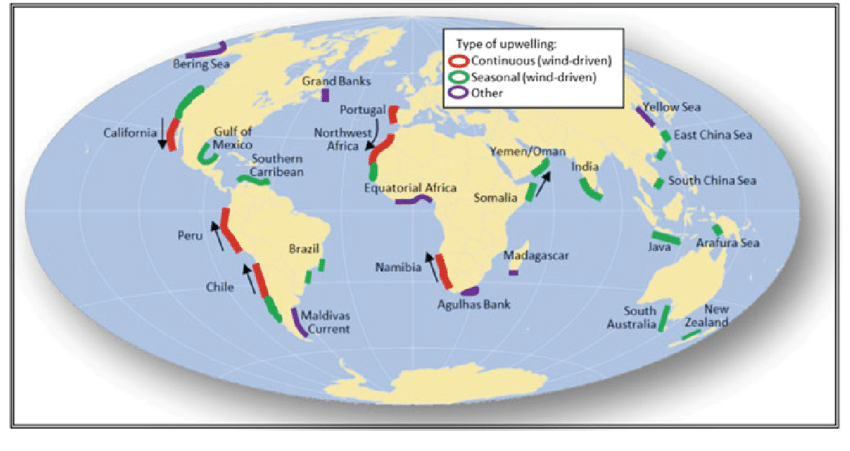
\includegraphics[scale=0.3]{../figures/M1/Locations-of-significant-coastal-upwelling-regions-in-the-world-ocean}

Upwelling regions in the world ocean. (Kaempf and Chapman, 2016, The
Functioning of Coastal Upwelling Systems, DOI: 10.1007/978-3-319-42524-5\_2,
In: Upwelling Systems of the World)
\end{frame}

\begin{frame}{Examples of using scalar products in oceanography}

\begin{columns}[t]


\column{8.5cm}
\begin{itemize}
\item {\small{}Longshore currents: most waves arrive at the shoreline with
an angle even if there is refraction. The component of the velocity
parallel to the coast obtained with the scalar product is the resulting
longshore (residual) current. The combination of residual currents
creates the dangerous rip currents.}{\small\par}
\item {\small{}Ekman-driven coastal upwelling: most of the winds incident
on coastlines can generate upwelling. There is always a wind component
along-shore. However, the eastern boundary upwelling regions }\textbf{\small{}are
more effective because the scalar product}{\small{} between the equatorward
wind vectors and coastal geometry }\textbf{\small{}is the largest}{\small\par}
\end{itemize}

\column{6cm}

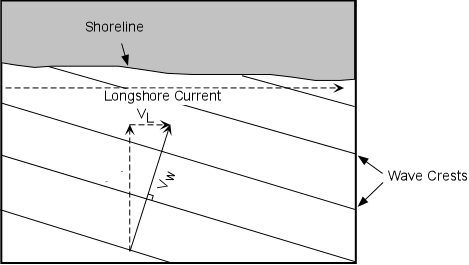
\includegraphics[width=6cm]{../figures/M1/longshore_current}

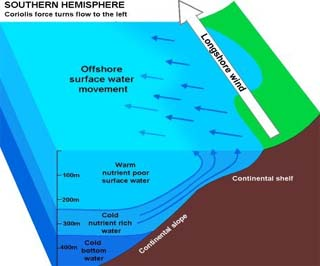
\includegraphics[scale=0.4]{../figures/M1/longshore_wind}
\end{columns}

\end{frame}

\begin{frame}{The dot product (aka scalar or inner product)}

\begin{itemize}
\item The \textbf{dot product} of 2 vectors \textbf{is a scalar}
\[
\mathbf{x}\cdot\mathbf{y}=\begin{bmatrix}x_{1} & x_{2} & x_{3}\end{bmatrix}\cdot\begin{bmatrix}y_{1}\\
y_{2}\\
y_{3}
\end{bmatrix}=x_{1}y_{1}+x_{2}y_{2}+x_{3}y_{3}
\]
\item It is \uline{commutative} $\mathbf{x}\cdot\mathbf{y}=\mathbf{y}\cdot\mathbf{x}$
\item If one of the vectors is of magnitude 1 (like the unit vectors), it
is geometrically interpreted as the length of the \emph{projection}
of one on the other when the two vectors are connected by the tails\\
\ \ \ \ \ \ \ 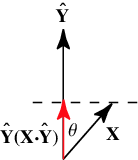
\includegraphics[scale=0.4]{../figures/M1/DotProduct}The
magnitude is $\mathbf{x}\cdot\mathbf{y}=\left\Vert \mathbf{x}\right\Vert \ \left\Vert \mathbf{y}\right\Vert \cos\theta$
\textbf{}\\
\textbf{Question: }\emph{What happens if the two vectors are orthogonal?}
\end{itemize}
\end{frame}

\begin{frame}{The cross product (vector product)}
\label{frame:cross-product}

\begin{itemize}
\item {\footnotesize{}The }\textbf{\footnotesize{}cross product}{\footnotesize{}
of two vectors is }{\footnotesize{}\uline{not commutative}}{\footnotesize{}
and }\textbf{\footnotesize{}the result is a vector}{\footnotesize{} }{\footnotesize\par}
\begin{enumerate}
\item {\footnotesize{}perpendicular to the plane on which the vectors lay
}\\
{\footnotesize{} 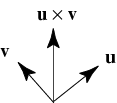
\includegraphics[scale=0.4]{../figures/M1/CrossProduct}}{\footnotesize\par}
\item {\footnotesize{}the magnitude is $\mathbf{u}\times\mathbf{v}=\left\Vert \mathbf{u}\right\Vert \ \left\Vert \mathbf{v}\right\Vert \sin\theta$ }{\footnotesize\par}
\item {\footnotesize{}the direction follows the right hand rule}{\footnotesize\par}
\end{enumerate}
\item {\footnotesize{}The geometric interpretation is less obvious, but
it can be thought as the area of the parallelogram between the vectors
\url{https://www.geogebra.org/m/eJHkAES2}. }\textbf{\footnotesize{}What
happens if the two vectors are orthogonal? }{\footnotesize\par}
\item {\footnotesize{}Deriving the components is a bit tricky. It's the
}\emph{\footnotesize{}determinant}{\footnotesize{} of a special matrix
in which the rows are the unit vectors and the multipliers, which
can be done with the }\emph{\footnotesize{}\href{https://en.wikipedia.org/wiki/Rule_of_Sarrus\#:~:text=Rule\%20of\%20Sarrus\%3A\%20The\%20determinant,along\%20the\%20up\%2Dright\%20diagonals.}{rule of Sarrus}}
\[
\!\!\!\mathbf{u\times}\mathbf{v}=\begin{vmatrix}\mathbf{\hat{i}} & \mathbf{\hat{j}} & \mathbf{\hat{k}}\\
u_{x} & u_{y} & u_{z}\\
v_{x} & v_{y} & v_{z}
\end{vmatrix}=\left(u_{y}v_{z}-u_{z}v_{y}\right)\mathbf{\hat{i}}-\left(u_{x}v_{z}-u_{z}v_{x}\right)\mathbf{\hat{j}}+\left(u_{x}v_{y}-u_{y}v_{x}\right)\mathbf{\hat{k}}
\]
\end{itemize}
\end{frame}

\begin{frame}{Example of vector products: angular momentum}

\begin{definition}
Angular momentum in physics is a measure of the amount of rotation
of an object. It is the rotational analogue of linear momentum (velocity
times mass, $\vec{p}=m\vec{V}$) but in this case it is referenced
to an origin (the axis/centre of rotation)
\[
\vec{L}=\vec{r}\times m\vec{V}
\]
\end{definition}

\begin{columns}[t]


\column{8cm}
\begin{itemize}
\item {\small{}Angular momentum is a vector that identifies the plane of
rotation and the quantity of motion}{\small\par}
\item {\small{}In fact, it is oriented as the angular velocity $\frac{d\theta}{dt}=\vec{\omega}$ }{\small\par}
\item {\small{}It can be demonstrated by first thinking about linear velocity
$\vec{V}=\vec{\omega}\times\vec{r}$ and computing the triple vector
product (see slide \ref{frame:useful})}{\small\par}
\end{itemize}

\column{6cm}

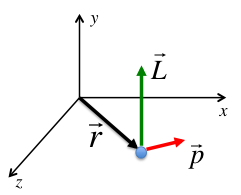
\includegraphics[width=5cm]{../figures/M1/angular_momentum}
\end{columns}

\end{frame}

\begin{frame}{Conservation of angular momentum}

\begin{definition}
In the absence of external forces (torque), \textbf{angular momentum
is conserved}. This is a basic principle for ocean and atmosphere
dynamics on a rotating Earth. Geophysical fluids conserve their initial
angular momentum given by the Earth rotation at their location if
there are no external forces in action
\end{definition}

\begin{columns}[t]


\column{6cm}
\begin{itemize}
\item The typical example of angular momentum and conservation is given
by a spinning figure skater: when the arms are contracted the spin
velocity increases
\end{itemize}

\column{6cm}

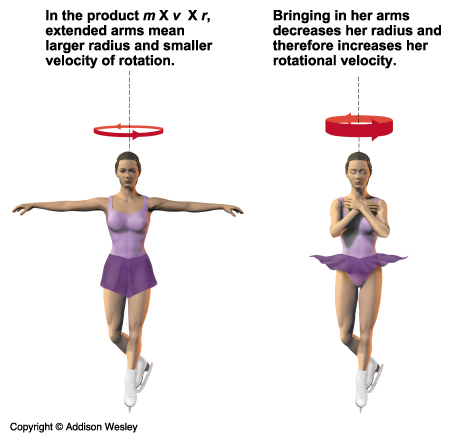
\includegraphics[width=4cm]{../figures/M1/skater}
\end{columns}

\end{frame}

\begin{frame}{Useful relationships}
\label{frame:useful}


\framesubtitle{spend some time to demonstrate them}
\begin{enumerate}
\item $\mathbf{\hat{i}}\cdot\mathbf{\hat{i}}=1;\ \mathbf{\hat{j}}\cdot\mathbf{\hat{j}}=1;\ \mathbf{\hat{k}}\cdot\mathbf{\hat{k}}=1$
\item $\mathbf{\hat{i}}\cdot\mathbf{\hat{j}}=0;\ \mathbf{\hat{j}}\cdot\mathbf{\hat{k}}=0;\ \mathbf{\hat{i}}\cdot\mathbf{\hat{k}}=0$
\item $\mathbf{\hat{i}}\times\mathbf{\hat{j}}=\mathbf{\hat{k}};\ \mathbf{\hat{j}}\times\mathbf{\hat{k}}=\mathbf{\hat{i}};\ \mathbf{\hat{i}}\times\mathbf{\hat{k}}=-\mathbf{\hat{j}}$
(1-3 demonstrate that the bases in the identity matrix are orthonormal)
\item $\mathbf{a}\times\mathbf{a}=0$
\item $\mathbf{a}\times\mathbf{b}=-\mathbf{b}\times\mathbf{a}$
\item $\mathbf{a}\cdot\left(\mathbf{a}\times\mathbf{b}\right)=0$
\item Triple scalar product: $\mathbf{a}\cdot\left(\mathbf{b}\times\mathbf{c}\right)=\mathbf{b}\cdot\left(\mathbf{c}\times\mathbf{a}\right)=\mathbf{c}\cdot\left(\mathbf{a}\times\mathbf{b}\right)$
\item Triple vector product: $\mathbf{a}\times\left(\mathbf{b}\times\mathbf{c}\right)=\mathbf{b}\mathbf{\left(a\cdot\mathbf{c}\right)-}\mathbf{c}\mathbf{\left(a\cdot\mathbf{b}\right)}$
\emph{(mnemonic: BAC-CAB. This relationship is used to demonstrate
that angular momentum is oriented as angular velocity)}
\end{enumerate}
\end{frame}

\begin{frame}{Working with matrices: linear transformations}

\begin{definition}
A linear transformation is a relationship that satisfies the following
rules
\begin{align*}
F\left(x+y\right) & =F\left(x\right)+F\left(y\right)\\
F\left(cx\right) & =cF\left(x\right)
\end{align*}
\end{definition}

\begin{itemize}
\item Vector-matrix multiplication in the 2-D plane is equivalent to a change
of coordinates. This is a linear transformation
\item A \textbf{symmetrical reflection} (along a point or axis) and \textbf{stretching}
are linear matrix transformation on the plane \emph{(this is exactly
what powerpoint or photoshop do when you flip or stretch an object
or a picture)}
\item A \textbf{rotation} is also a linear transformation involving a vector-matrix
product
\item Learn more about matrix transformations here \url{https://www.khanacademy.org/math/linear-algebra/matrix_transformations}
\end{itemize}
\end{frame}

\begin{frame}[fragile]{Example 1.5.1 - Stretching plane figures}

\begin{itemize}
\item {\footnotesize{}Through the vector-matrix product it is possible to
flip and stretch an object }\emph{\footnotesize{}(Note: a shift is
simply the addition of constants to the coordinates)}{\footnotesize\par}
\item {\footnotesize{}An ordered array is also called an }\textbf{\footnotesize{}n-tuple}{\footnotesize{}.
A figure on the plane can be seen as a set of pairs or 2-tuples }\emph{\footnotesize{}(Note:
to graphically ``connect the dots'' and close a polygon we need
to connect the last point with the first point, hence we repeat the
pair). }{\footnotesize\par}
\item \emph{\footnotesize{}Try these lines of code on Matlab (the figure
will not look identical):}{\footnotesize{} }{\footnotesize\par}
\end{itemize}
\begin{columns}[t]


\column{7cm}

\begin{lstlisting}[language=Matlab,basicstyle={\scriptsize},breaklines=true]
>> figure
>> triangle=[1 3 1 1; 3 3 -1 3]
triangle =
     1     3     1     1
     3     3    -1     3
>> line(triangle(1,:),triangle(2,:))
>> axis([-8 8 -8 8])
>> set(gca,'xtick',-8:8,'ytick',-8:8)
>> grid on
\end{lstlisting}


\column{6.5cm}

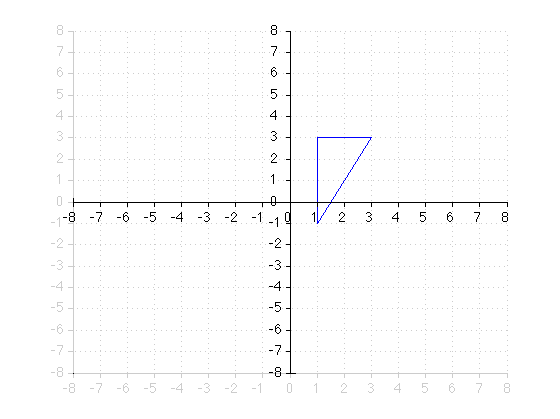
\includegraphics[scale=0.3]{../figures/M1/triangle}
\end{columns}

\end{frame}
%
\begin{frame}{Linear transformation of coordinates (I)}
\begin{itemize}
\item Let's assume we are looking for a function $t$ that changes any object
on the Cartesian plane to another one that is flipped with respect
to the y-axis and it's magnified 2 times along the $y$ direction. 
\item This is equivalent to changing the sign of the coordinate $x$ and
doubling the coordinate $y$. \emph{(Note: spend some time to think
about it, and if you don't see it, go straight to the code in the
next slide and then come back to the math)}
\[
t:\begin{bmatrix}x\\
y
\end{bmatrix}\mapsto\begin{bmatrix}-x\\
2y
\end{bmatrix}
\]
\end{itemize}
\end{frame}

\begin{frame}[fragile]{Linear transformation of coordinates (II)}

\begin{columns}[t]


\column{8.5cm}
\begin{itemize}
\item {\small{}To write the transformation matrix, we apply this function
to the columns of the identity matrix $I_{2}$, i.e. the base of our
coordinate system. }\emph{\small{}(Note: go back to eq. \ref{eq:identity-matrix}
in Section 1.4 if the relationship between the identity matrix and
the coordinate system is not clear)}{\small{}:
\[
\mathbf{T}=\left[t\left(\begin{bmatrix}1\\
0
\end{bmatrix}\right)\ t\left(\begin{bmatrix}0\\
1
\end{bmatrix}\right)\right]=\begin{bmatrix}-1 & 0\\
0 & 2
\end{bmatrix}
\]
}{\small\par}
\item {\small{}Thanks to the matrix $\mathbf{T}$, every point of our triangle
(i.e. a vector on the 2D plane) can be transformed using a vector-matrix
product
\[
t\left(\mathbf{x}\right)=\mathbf{Tx}=\begin{bmatrix}-1 & 0\\
0 & 2
\end{bmatrix}\cdot\begin{bmatrix}x\\
y
\end{bmatrix}
\]
} 
\end{itemize}

\column{6.5cm}

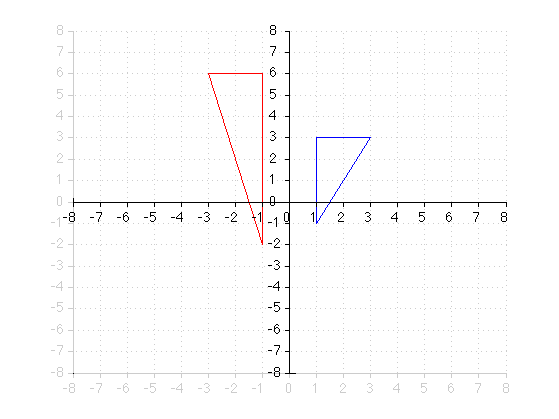
\includegraphics[width=5cm]{../figures/M1/triangle_T}

\begin{lstlisting}[language=Matlab,basicstyle={\tiny},breaklines=true]
>> T=[-1 0;0 2]
 T =
    -1     0
     0     2
>> tt=T*triangle
 tt =
    -1    -3    -1    -1
     6     6    -2     6
>> h=line(tt(1,:),tt(2,:),'color','r')
\end{lstlisting}

\end{columns}

\end{frame}

\begin{frame}{Example 1.5.2 - Rotating vector objects}

\begin{columns}[t]


\column{9cm}
\begin{itemize}
\item {\footnotesize{}The rotation by an angle $\theta$ is also a }\emph{\footnotesize{}linear
transformation}{\footnotesize{} and can be expressed via vector-matrix
products}{\footnotesize\par}
\item {\footnotesize{}As done for the previous case, we can derive the transformation
matrix through the transformation of the coordinate bases $I_{2}$
\[
\mathbf{R_{\theta}}=\left[rot_{\theta}\left(\begin{bmatrix}1\\
0
\end{bmatrix}\right)\ rot_{\theta}\left(\begin{bmatrix}0\\
1
\end{bmatrix}\right)\right]
\]
}{\footnotesize\par}
\item {\footnotesize{}The resulting matrix can be obtained graphically using
the trigonometric functions }\emph{\footnotesize{}(Note, check the
Kahn Academy video for the full derivation)}{\footnotesize{}. This
leads to the generic form of a rotation matrix
\[
\mathbf{R_{\theta}}=\begin{bmatrix}\cos\theta & -\sin\theta\\
\sin\theta & \cos\theta
\end{bmatrix}\ \textrm{and }\mathbf{v}'=\mathbf{R}_{\theta}\mathbf{v}_{0}
\]
}{\footnotesize\par}
\end{itemize}

\column{5cm}

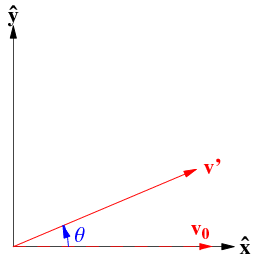
\includegraphics[scale=0.3]{../figures/M1/RotationVector}

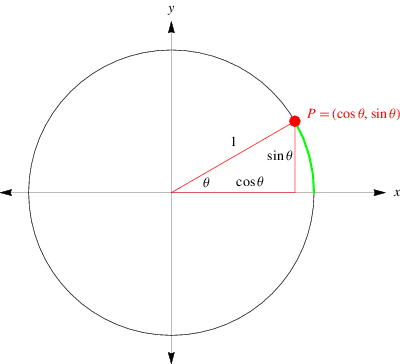
\includegraphics[scale=0.3]{../figures/M1/TrigonometryUnitCircle}
\end{columns}

\end{frame}

\begin{frame}{Example 1.5.3 - Working with matrices to solve linear systems}

\begin{columns}[t]


\column{7.5cm}
\begin{itemize}
\item You are a scientist studying marine mammals. As part of your research,
you need to tag a bottlenose dolphin with a GPS tracker. You are on
a small boat at about 10 km from the coast.
\item Bottlenose dolphins are very rapid swimmers, with a speed up to 10
m/s. This is unfortunately the maximum speed of your boat
\item The dolphin is currently swimming at 8 m/s and you need to wait 2
minutes to calibrate the GPS before running
\end{itemize}

\column{7cm}

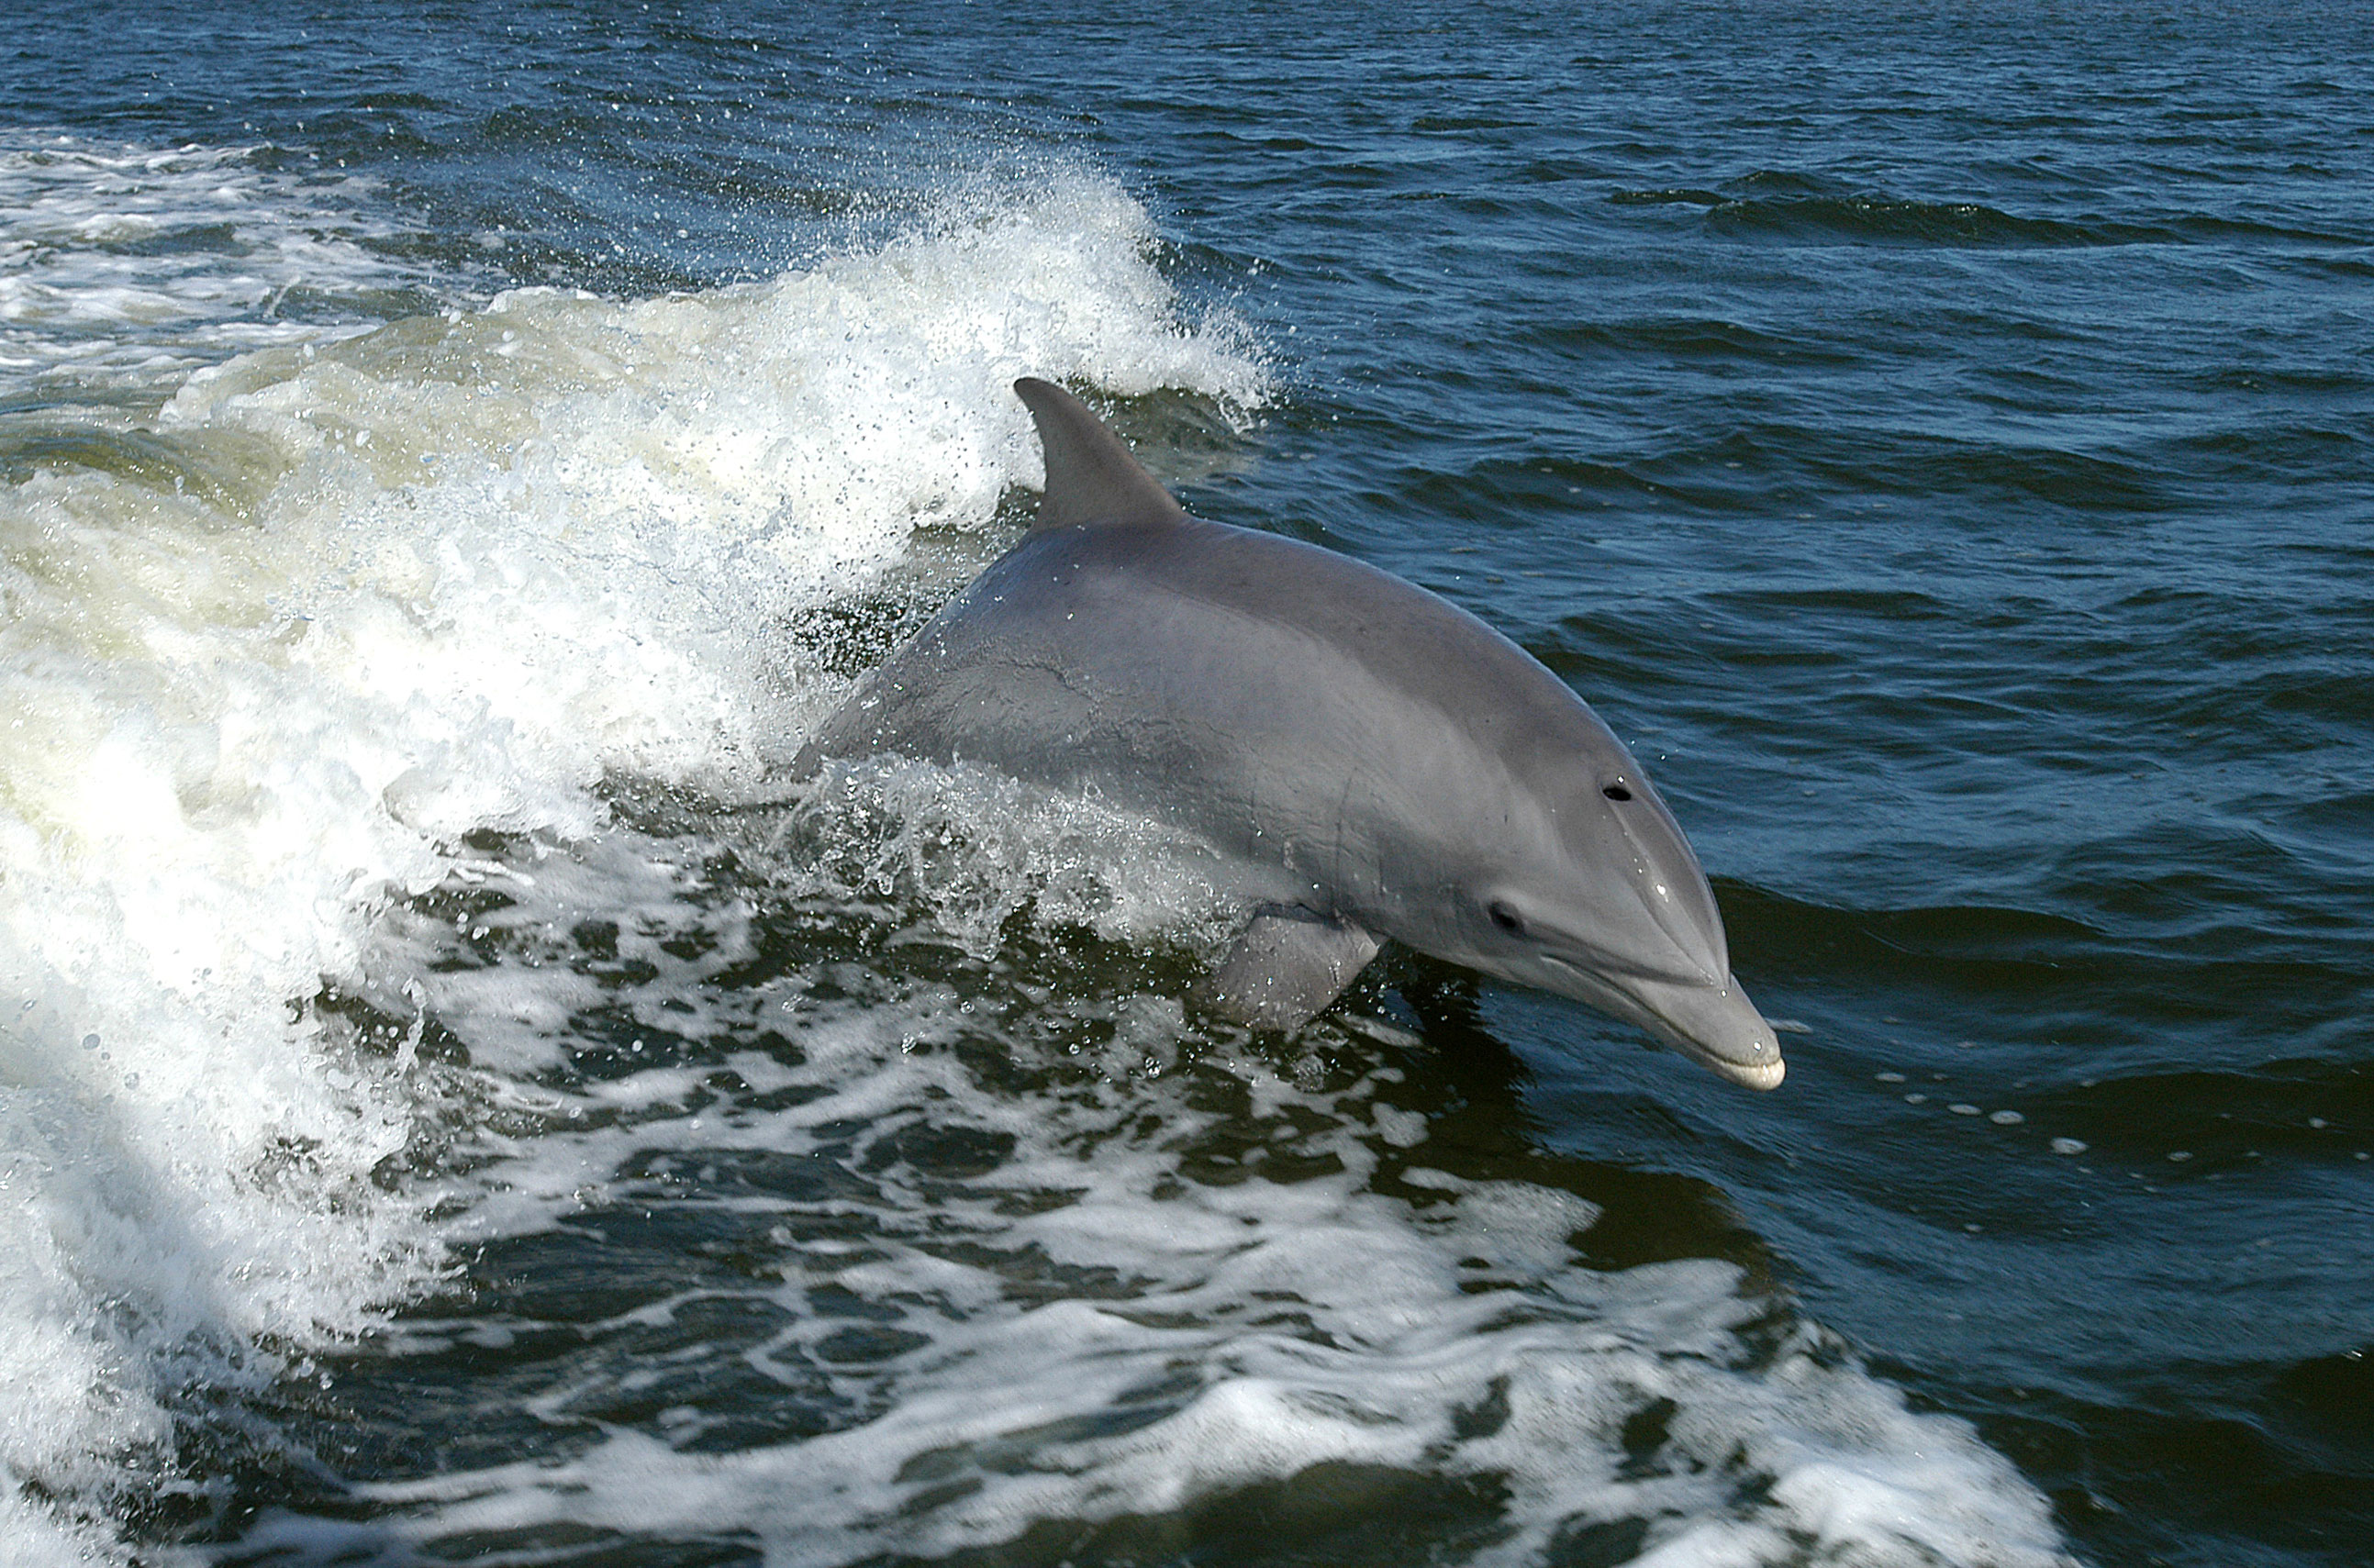
\includegraphics[scale=0.07]{../figures/M1/Bottlenose_Dolphin}

\textbf{Will you be able to reach the dolphin before it gets too close
to the coast?} 

This problem is a typical \emph{linear system of equations} and the
solution is a matter of seconds with a computer
\end{columns}

\end{frame}

\begin{frame}{Solving a linear system (I)}

\begin{itemize}
\item The problem can be written in the following terms
\begin{align*}
x & =V_{d}t\\
x & =V_{b}\left(t-T_{gps}\right)
\end{align*}
where $V_{d}$ and $V_{b}$ are the speeds of the dolphin and the
boat (8 and 10 m/s, respectively). $T_{gps}$ is the time needed to
set the GPS (2 min = 120 s) and $x,\ t$ are the unknowns, the distance
and the time of the encounter
\item One can solve this by substitution of variables as you learned at
high school, but linear algebra is much more effective. The equations
can be written in terms of vectors and one transformation matrix:
\[
\begin{cases}
x-V_{d}t & =0\\
x-V_{b}t & =-V_{b}T_{gps}
\end{cases}\Rightarrow\begin{bmatrix}1 & -V_{d}\\
1 & -V_{b}
\end{bmatrix}\cdot\begin{bmatrix}x\\
t
\end{bmatrix}=\begin{bmatrix}0\\
-V_{b}T_{gps}
\end{bmatrix}\Rightarrow\mathbf{Ax}=\mathbf{c}
\]
\end{itemize}
\end{frame}

\begin{frame}[fragile]{Solving a linear system (II)}

\begin{columns}[t]


\column{7cm}
\begin{itemize}
\item {\footnotesize{}The solution of a linear system with linear algebra
is very similar to solving the equation $ax=c\Rightarrow x=\frac{1}{a}c=a^{-1}c$}{\footnotesize\par}
\item {\footnotesize{}Is there such a thing like the inverse of a matrix?
YES!}{\footnotesize\par}
\item {\footnotesize{}The solution of $\mathbf{Ax}=\mathbf{c}$ is the matrix
$\mathbf{B}$ that satisfies $\mathbf{x}=\mathbf{Bc}$, and this is
the inverse of $\mathbf{A}$. }{\footnotesize\par}
\end{itemize}

\column{8cm}
\begin{itemize}
\item {\footnotesize{}There is no need to know how to invert a matrix by
hand. Try this in Matlab}{\footnotesize\par}
\item 
\begin{lstlisting}[language=Matlab,basicstyle={\tiny}]
>> A=[1 -8; 1 -10]
A =
     1    -8
     1   -10
>> c=[0; -120*10]
c =
           0
       -1200
>> B=inv(A)
B =
    5.0000   -4.0000
    0.5000   -0.5000
>> x=B*c
x =
        4800
         600
\end{lstlisting}
\end{itemize}
\end{columns}

\begin{definition}
{\footnotesize{}The inverse of a matrix must satisfy the relationship
$\mathbf{BA}=\mathbf{I}$, i.e. the product of a matrix by its inverse
is equal to the identity matrix: $\mathbf{A^{-1}A}=\mathbf{I}$}{\footnotesize\par}
\end{definition}

\end{frame}

\end{document}
